\chapter{Creating a graphene kirigami system}\label{chap:system}

The system definition plays an essential role in the ``friction experiment''
that we are going to carry out through \acrshort{MD} simulations. The purpose of
the simulations is to quantify the friction that arises when a stretched
Kirigami graphene sheet slides over a substrate. We aim to design the simplest
possible system that allows for such a measurement under variations of Kirigami
design, strain and load.

For this purpose, two approaches were considered as sketched in
\cref{fig:system_variations}. One approach is simply to mimic a \acrshort{FFM}
type experiment where the graphene sheet is resting on a substrate and a moving
body scans across the graphene surface as seen in~\cref{fig:system_variation_b}.
This setup allows for a variety of tip designs, and we can even substitute the
tip for a flat surface making the setup resemble a \acrshort{SFA} experiment
instead. For this setup, we would attach a pre-stretched sheet to the substrate
and require the edges of the sheet to be fixated on the substrate to sustain the
stretch. Thus, the sheet and substrate would constitute the manufactured object
and the moving body would represent the contact to the outside world. In this
approach, the potential applications would relate to certain effects being
associated with a constant strain value. Another approach is to have the sheet
ends fixated on the moving body instead as shown in
\cref{fig:system_variation_a}. This switches the roles of the involved parts as
we now view the moving body and the sheet as the manufactured object
while contact with the substrate represents the outside world. This allows
for the introduction of a nanomachine design that converts the load to a strain of the of the sheet. Thus, the possible applications allow for a dynamic effect
with changing strain through the loading of the sheet. While both methods serve
as novel approaches with prospects of providing valuable insight into a sparsely
covered field, we choose the latter option (\cref{fig:system_variation_a}) due to the increased application possibilities.

We do not attempt to model the nanomachine explicitly, but we will use the
conceptual idea of a coupling between load and strain to motivate our study. Hence our system of choice consists of a 2D graphene sheet with locked ends, mimicking
the attachment to a moving body, and a 3D silicon bulk substrate. 


\begin{figure}[h]
  \centering
  \begin{subfigure}[b]{0.49\textwidth}
    \centering
    \includegraphics[width=\textwidth]{figures/system/system_variations_a.png}
    \caption{}
    \label{fig:system_variation_a}
  \end{subfigure}
  \hfill
  \begin{subfigure}[b]{0.49\textwidth}
    \centering
    \includegraphics[width=\textwidth]{figures/system/system_variations_b.png}
    \caption{}
    \label{fig:system_variation_b}
  \end{subfigure}
  \hfill
  \caption{Conceptual visualization of two different system setups considered. The wiggly line represents the Kirigami sheet. (a) The chosen setup with a manufactured object connected to the sheet. The contact with the substrate represents the contact with the outside world. (b) An alternative setup where the sheet is fixed in the substrate constituting the manufactured object. The contact with the outside world is then represented through an indention by objects with various shapes and sizes. }
  \label{fig:system_variations}
\end{figure}

% \begin{figure}[h]
%   \centering
%   \includegraphics[width=0.8\linewidth]{figures/system/system_variations.png}
%   \caption{\hl{TMP} System variations}
%   \label{fig:system_variations}
% \end{figure}





% Note that the rigid parts on both sides of the
% sheet is then considered as a single rigid object even though they are
% physically seperated. This means that all force interactions concerning the
% rigid parts will be applied as a common average making them move in total
% synchronization. 


\section{Region definitions}
We subdivide the two main parts of the system, the sheet and the substrate, into
specific regions according to their functionality in the \acrshort{MD}
simulations. For the sheet, we denote a subsection of the ends, with respect to
the sliding direction, as so-called \textit{pull blocks}, which is reserved for
the application of normal load, stretching, dragging of the sheet, and for
applying the thermostat. The remaining \textit{inner sheet} is left for the
Kirigami cuts and is simulated as an $NVE$ ensemble. This partitioning is motivated by the idea that we want to minimize direct manipulations on the inner sheet, given its presumed critical role in governing friction behavior. The pull blocks are
equally split between a thermostat part and a rigid part. It should be noted that the rigidness of the pull blocks is enforced only after a relaxation period to ensure that the crystal structure is fully relaxed. This is further explained in~\cref{sec:num_proc}. The substrate is equally divided into three parts: The
\textit{upper layers} ($NVE$) responsible for the sheet-substrate interaction,
the \textit{middle layers} being a thermostat ($NVT$), and the \textit{bottom
layers} being frozen, made rigid and fixed, in the initial lattice structure to
ensure that the substrate stays in place. \cref{fig:system} show the system is
displayed with colors matching the three distinct roles:
\begin{enumerate}
  \item Red: $NVE$ parts which are governing the frictional behavior of interest.
  \item Green: Thermostats ($NVT$) surrounding the $NVE$ parts in order to modify the temperature without making disturbing changes to the interaction of the sheet and substrate.
  \item Blue: Parts that are initially or eventually turned into rigid objects. For the substrate, this refers to an additional fixation as well.
\end{enumerate}
The full sheet is given a size $\sim 130 \times \SI{163}{\text{Å}}$ while the substrate is scaled accordingly to the sheet which is further specified in~\cref{sec:substrate}. For an expected strain of 200\% the total system size is roughly \num{55e3} atoms. The specific distribution of atoms is shown in \cref{tab:system_count} along with the spatial x-y-measures in \cref{tab:sheet_dim}. An example of a strained sheet is shown in~\cref{fig:kirigami_stretch}


\begin{figure}[h]
  \centering
  \begin{subfigure}[b]{0.60\textwidth}
      \centering
      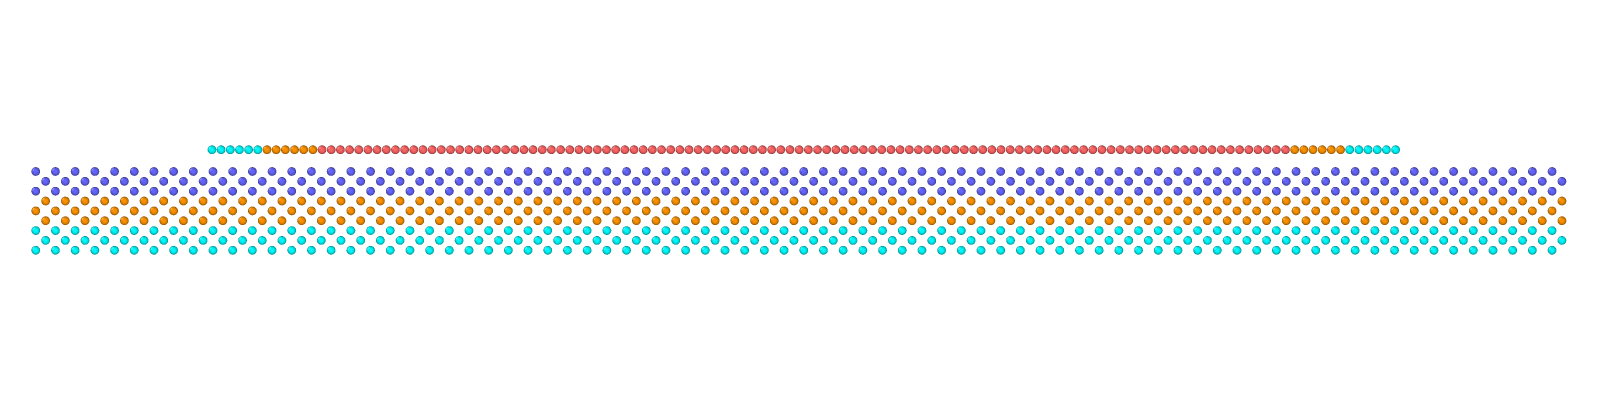
\includegraphics[width=\textwidth]{figures/system/system_sideview.png}
      \caption{}
      \label{fig:sideview}
  \end{subfigure}
  \hfill
  \begin{subfigure}[b]{0.60\textwidth}
      \centering
      \includegraphics[width=\textwidth]{figures/system/system_topview_anno.png}
      \caption{}
      \label{fig:topview}
  \end{subfigure}
  \hfill
     \caption{System configuration colorized to indicate NVE parts (red), thermostat parts (green) and rigid parts (blue). (a) Side view showing the sheet on top of the substrate. (b) Top view showing only the sheet}
     \label{fig:system}
\end{figure}


\begin{figure}[h]
  \centering
  \includegraphics[width=0.7\linewidth]{figures/system/hon_stretch.png}
  \caption{Stretched Kirigami sheet against a substrate. The substrate is excluded from the image for better visibility. The atoms are coloredized to indicate NVE parts (red), thermostat parts (green) and rigid parts (blue). The pattern used is the Honeycomb $(2,2,1,5)$ (see \cref{chap:system}) at a 100\% strain level.}
  \label{fig:kirigami_stretch}
\end{figure}


\begin{table}[h]
  \begin{center}
  \caption{Specification of the spatial size of the system for the x-y-dimensions with a substrate scaled for an expected sheet strain of 200\%. The first column denotes the size relative to the full sheet size $x_S \times y_S$, while the second column denotes the corresponding length in Å.}
  \label{tab:sheet_dim}
  \begin{tabular}{ | l | r@{}l | r@{}l | c |} \hline
    \textbf{Region} & \multicolumn{2}{c|}{Dim} & \multicolumn{2}{c|}{Dim
    [Å]} & Area [nm$^2$]\\ \hline
  Full sheet & $x_S \: \times \: $ & $y_S$ &  $130.029 \: \times \:$ & $163.219$ Å & $\phantom{2\times} 212.23$ \\ \hline
  Inner sheet & $x_S \: \times \:$ & $0.81 \ y_S$ &  $130.029  \: \times \:$ & $132.853$ Å & $\phantom{2\times} 172.74$\\ \hline
  Pull blocks & $2 \times x_S \: \times \:$ & $ 0.09 \ y_S$ & $2 \times 130.029  \: \times \: $ & $\phantom{0}15.183$ Å  & $2 \times \phantom{0}19.74$ \\ \hline  
  Substrate & $1.16 \ x_S \: \times \:$ & $3.12 \ y_S$ &  $150.709  \: \times \:$ & $509.152$ Å & $\phantom{2\times} 767.34$\\ \hline
\end{tabular}
\end{center}
\end{table}



\begin{table}[h]
  \begin{center}
  \caption{Specification of the system size regarding the number of atoms for various system regions. These numbers correspond with the case of no cuts applied to the sheet and a substrate scaled for the expected stretch of 200\%.}
  \label{tab:system_count}
  \begin{tabular}{ |c?{0.3mm} c | c | c | c | c | c |} \hline
    \textbf{Region} & \textbf{Total}  & Sub region & Sub total & \textbf{NVE} &
    \textbf{NVT} & \textbf{Rigid} \\ \hline   
    \multirow{2}{*}{Full sheet} & \multirow{2}{*}{7800} & Inner sheet & 6360 & 6360 &
    0 & 0 \\ %\hline
    & & Pull blocks & 1440 & 0 & 720 & 720 \\ \hline   
    \multirow{3}{*}{Substrate} & \multirow{3}{*}{47376} & Upper & 15792 & 15792 &
    0 & 0 \\ %\hline
    & & Middle & 15792 & 0 & 15792 & 0 \\ %\hline
    & & Bottom & 15792 & 0 & 0 & 15792 \\ \Xhline{2\arrayrulewidth}   
    All & 55176 & \multicolumn{2}{r|}{} & 22152 & 16512 & 16512 \\ \hline 
  \end{tabular}
  \end{center}
\end{table}


\section{Numerical procedure}\label{sec:num_proc}
Following the system setup as described previously, the next step involves letting the system relax and reach a stable equilibrium. During this phase, slight modifications to the sheet-substrate distance and lattice spacing take place, both of which are influenced by the thermostat's target temperature. We then stretch the sheet to the desired length, apply normal load and finally slide it along the substrate. The full numerical procedure can be arranged into the following steps. Some steps have been given a default duration denoted in parentheses in units of ps, \num{e-12} seconds.
\begin{enumerate}
  \item \textbf{Relaxation} (\SI{15}{ps}): The sheet and substrate are relaxed for 
  \SI{15}{ps} after being added in their crystalline form with a separation distance of \SI{3}{\text{Å}}. Given that the equilibrium separation distance will vary with temperature, this value is based on an average estimate suiting our temperature range of interest. In order to avoid any sheet drift we constrain it with the use of three hard spring forces with a spring constant
  $\SI{e5}{eV/\text{Å}^2} \sim \SI{1.6e6}{N/m}$: One spring attaches the sheet center of mass (\acrshort{CM}) to its original position, preventing \acrshort{CM} drift, while the remaining two springs are attached to the pull blocks \acrshort{CM}, to prevent rotation. In principle, fixing only one of the pull blocks would suffice, but we choose to fixate both to maintain symmetry. During the relaxation phase, we consider the pull blocks to be rigid with respect to the z-direction only (perpendicular to the sheet). That is, all the forces in the z-direction are summed up and applied as a uniform external force, while the pull blocks are free to expand and contract in the x-y-plane. This feature is incorporated to allow the sheet pull blocks to readjust the lattice spacing according to the temperature of the system. For the following steps, the pull blocks are made truly rigid with respect to all directions, and the spring forces are terminated. 
  \item \textbf{Stretch}: To stretch the sheet, the two opposing rigid parts of the pull blocks are moved apart at a constant velocity until the desired strain level is achieved. The duration of this phase is determined by the values of the \textit{stretch speed} and \textit{stretch amount} parameters.
  \item \textbf{Pause} (\SI{5}{ps}): The sheet is relaxed for \SI{5}{ps} to ensure that the sheet is stable and equilibrated after the applied strain deformation. 
  \item \textbf{Normal load} (\SI{5}{ps}): The pull blocks are subjected to a uniformly applied load in the negative z-direction, thereby pushing the sheet perpendicularly into the substrate. Initially a viscous damping force, $F = -\gamma \vec{v}$ with damping factor $\gamma$ and velocity $v$, is added to resist rapid acceleration of the sheet and prevent a hard impact between the sheet and substrate. The damping coefficient is set to $\gamma = \SI{8e-4}{nN/(m/s)}$ and terminated after \SI{0.5}{ps} which was found to be suitable for the extreme load cases of our intended range. The remaining \SI{4.5}{ps} is devoted to further relaxation in order to reach a sheet-substrate distance equilibrium.
  \item \textbf{Sliding}: A virtual atom is introduced into the simulation which
  exclusively interacts with the rigid parts of the pull blocks through a spring force with spring constant $K$ in the x-y-plane. The force in the z-direction is not influenced by the spring force and is instead governed by the equilibrium between the normal load and the normal response from the sheet-substrate interaction. The virtual atom is immediately given a constant velocity, given by the \textit{sliding speed} parameter. This results in an initial linear increase in sliding force proportional to sliding speed and spring constant $F_{\textit{slide}} \propto Kv_{\text{slide}}t$. An infinite spring constant can also be enforced for which the spring is omitted and the pull blocks are moved rigidly with a constant speed.
\end{enumerate}
To limit the complexity of the friction behavior we want to consider systems without wear. To make sure that no wear is taking place for the sheet, we monitor the nearest neighbors for each atom throughout the simulation. At the initial timestep the three nearest neighbors, sitting at a distance \SI{1.42}{\text{Å}}, of all graphene atoms are recorded. If any of these nearest neighbors exceeds a threshold distance of \SI{4}{\text{Å}}, indicating a bond breakage, this is marked as a rupture and we halt the simulation. By conducting several test simulations involving high loads and sliding speeds, we have visually confirmed that no wear occurs in the substrate, which demonstrates significantly greater wear resistance than the sheet. Therefore, we do not need to monitor the substrate for any signs of wear.


\section{Setting up the substrate}\label{sec:substrate}
The substrate is created as a rectangular slab of Silicon (Si). We create the
initial configuration according to its crystalline structure given as a diamond
cubic crystal with a lattice parameter $a_{\text{Si}} = \SI{5.43}{\text{Å}}$.
The default substrate thickness is chosen such that 9 layers of atoms appear (2
unit cells) corresponding to a thickness of \SI{10.86}{\text{Å}}. The x-y
dimensions are chosen to match the dimensions of the sheet. That is, we define a
margin between the sheet edge and the substrate edge for the x- and y-direction
respectively. Since we use periodic boundary conditions a too small margin would
result in the sheet edges interacting with themselves through the boundary. The
absolute lower limit for the margin choice is half the cut-off distance for
the Tersoff potential, governing the graphene sheet interaction, at $R + D =
\SI{2.1}{\text{Å}}$. However, due to fluctuations in the sheet, we cannot set the margin too
close to that limit. In addition, we need to consider the buckling of the sheet as it is stretched, which might cause an expansion in the x-direction for certain configurations. We choose an x-margin of \SI{20}{\text{Å}} which provides $2\cdot
\SI{20}{\text{Å}} - \SI{2.1}{\text{Å}} = \SI{37.9}{\text{Å}}$ of additional
spacing with respect to the absolute lower limit. By looking over the simulation
result visually we confirm that this leaves more than enough room in the cases
of extreme buckling. For the y-direction the rigid parts of the pull-blocks
moves a certain distance based on the strain value exclusively, and we define
the y-margin based on the remaining distance to the edge after stretching.
However, as the sheet travels through the periodic boundaries in the y-direction
when sliding, we want to add some additional spacing through the y-margin in
order to let the substrate surface relax before interacting with the sheet a
second time. We choose a y-margin of \SI{15}{\text{Å}} for which the preferred sliding speed
of $\SI{20}{m/s} = \SI{2}{\text{Å}/ps}$ gives \SI{15}{ps} of relaxation time
between encounters with the sheet, similar to the initial relaxation time. 


\section{Setting up sheet}
% \subsection{Graphene}
% (https://community.wvu.edu/~miholcomb/graphene.pdf)
% https://www.physics-in-a-nutshell.com/article/4/lattice-basis-and-crystal

The sheet consists of graphene, which is a single layer of carbon atoms arranged in a hexagonal lattice structure. The bulk version of graphene is graphite and is a stacked structure of multiple graphene layers. We can describe the graphene 2D crystal structure in terms of its primitive lattice vectors $\vec{a_1}$ and $\vec{a_2}$ and a basis. The basis describes the atoms associated with each lattice site, and we populate the lattice by translating the basis by any linear combination of the lattice vectors 
\begin{align*}
  \vec{T}_{mn} = m\vec{a_1} + n\vec{a_2}, \qquad m,n \in \mathbb{N}.
\end{align*}
For graphene, we have the primitive lattice vectors~\cite{gray2009crystal} 
\begin{align}
  \vec{a_1} = a \left(\frac{\sqrt{3}}{2}, -\frac{1}{2}\right), \qquad \vec{a_2} = a \left(\frac{\sqrt{3}}{2}, \frac{1}{2}\right), \qquad |\vec{a_1}| = |\vec{a_2}| = a = 2.46 \ \text{Å}.
  \label{eq:prim_vec}
  %, \qquad |\vec{a_1}| = |\vec{a_2}| = 2.46 \ \text{Å}.
\end{align}
Notice that we deliberately excluded the third coordinate as we only consider a
single graphene layer and thus we do not have to consider the stacking structure of 3D graphite. The basis consists of two carbon atoms given as 
\begin{align}
  \Big\{\Big(0,0\Big), \frac{a}{2}\Big(\frac{1}{\sqrt{3}}, 1 \Big) \Big\}.
  \label{eq:basis}
\end{align}
The crystal structure is visualized in \cref{fig:graphene_crystal}. The hexagonal lattice structure makes for an equal spacing all pairs of atoms with an interatomic distance
\begin{align*}
  \left|\left|\frac{a}{2}\Big(\frac{1}{\sqrt{3}}, 1 \Big)\right|\right| \approx 1.42 \ \text{Å}.
\end{align*}


\begin{figure}[h]
  \centering
  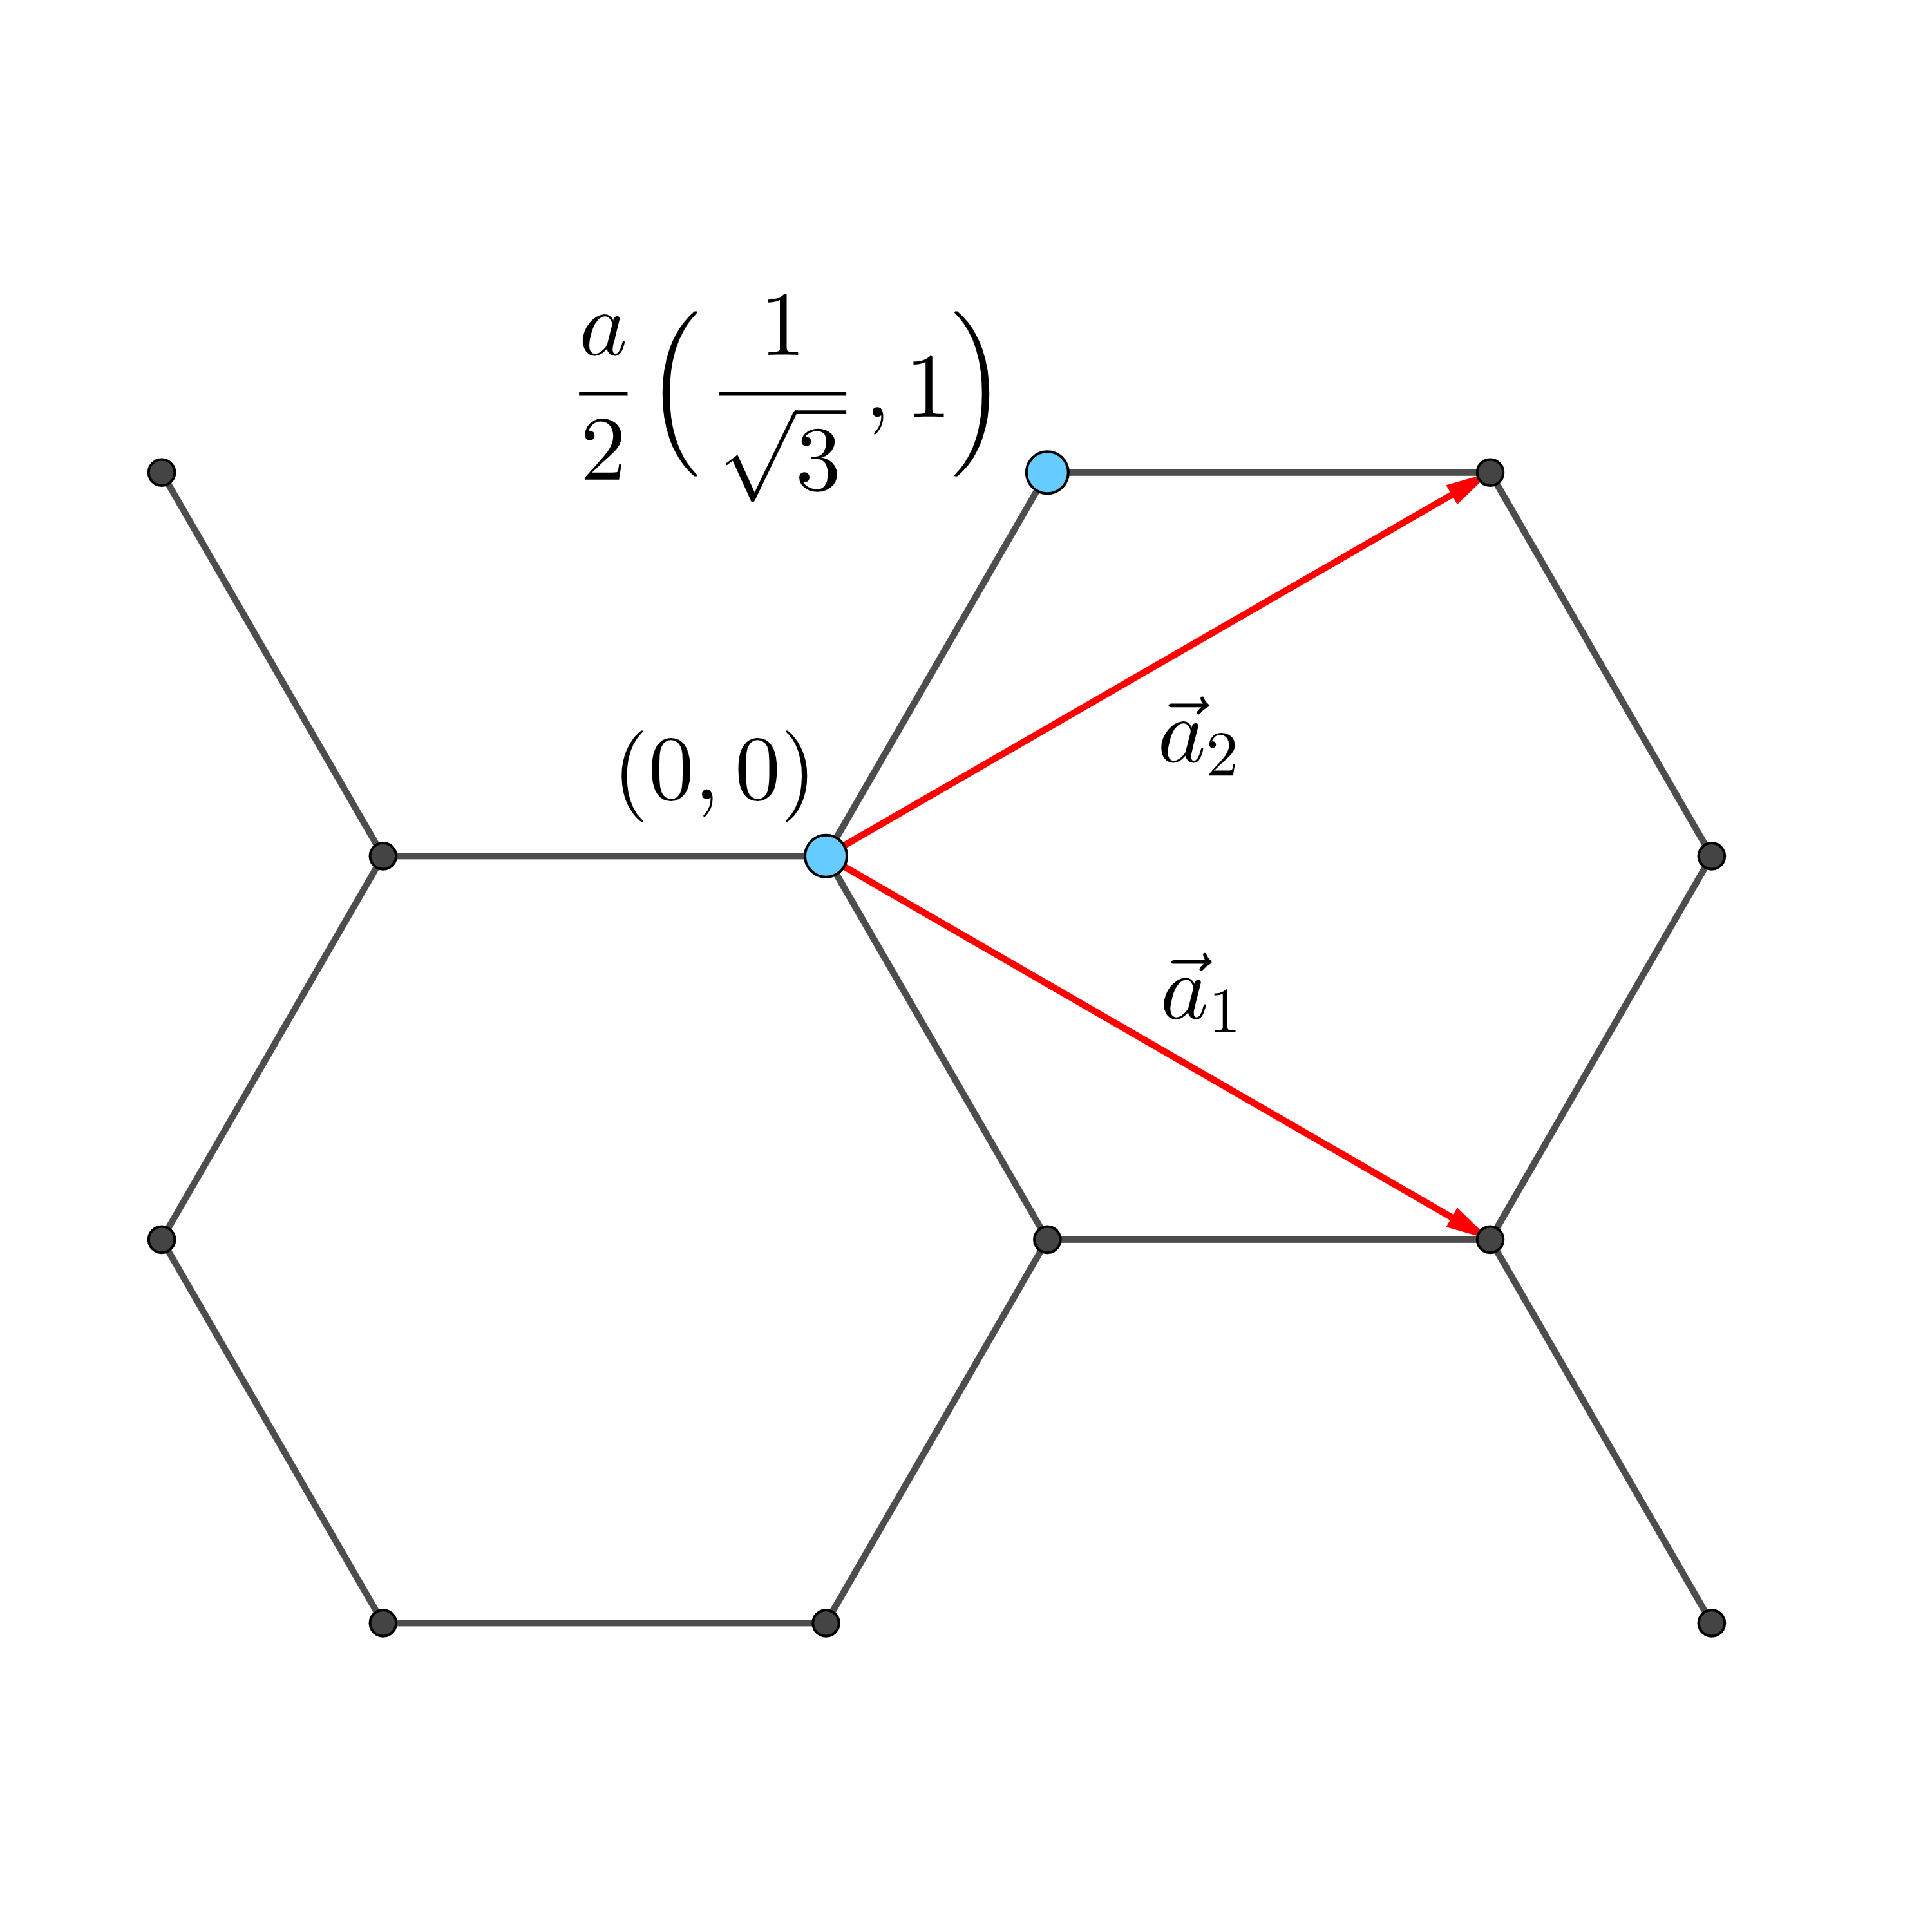
\includegraphics[width=0.3\linewidth]{figures/system/crystal.png}
  \caption{Illustration of the graphene crystal structure. The dots represent atom sites, blue dots denote the basis atoms (\cref{eq:basis}) and the red arrows denote the primitive lattice vectors (\cref{eq:prim_vec}). }
  \label{fig:graphene_crystal}
\end{figure}



\subsection{Indexing}
In order to describe the Kirigami cut patterns applied to the graphene sheet we require an indexing system that provides a unique representation of the atoms in the lattice. This allows us to represent the pattern as a binary matrix, where 0 denotes removed atoms and 1 denotes present atoms. We let the x-coordinate correspond with the so-called \textit{armchair} direction of the sheet and the y-coordinate with the so-called \textit{zigzag} direction. Notice that the x-coordinate will point to \textit{zigzag} chains of atoms for which the starting point $(x, 0)$ is not evenly spaced as illustrated in~\cref{fig:atom_indexing}. Other
solutions might naturally involve the lattice vectors, but since these are used
to translate between similar basis atoms it introduces an unfortunate duality as
one would then need to include the basis atom of choice into the indexing system
as well. Additionally, we want an indexing system that conserves the relative
physical position of neighbors. That is, atom $(i, j)$ should be in the
proximity of $\{(i+1, j), (i-1, j), (i, j+1), (i, j-1)\}$. However, due to the
hexagonal structure of the lattice, only three said neighbor indexes will be
actual nearest neighbors in the lattice. While $(i, j\pm 1)$ is always the nearest
neighbor, the index of the nearest neighbor in the x-direction oscillates for
each incrementing of the x- or y-coordinate. That is, the nearest neighbors \acrshort{NN} are decided as
\begin{equation}
  \begin{aligned}
    (i + j) \ \text{is even} &\rightarrow \text{\acrshort{NN}} = \{(i-1, j), (i, j+1), (i, j-1)\}, \\
    (i + j) \ \text{is odd} &\rightarrow \text{\acrshort{NN}} = \{(i+1, j), (i, j+1), (i, j-1)\}.
  \end{aligned}
  \label{eq:atom_neigh_idx}
\end{equation}
We can visually verify this by consulting~\cref{fig:atom_indexing}, which shows that the nearest neighbor indexes depend on whether the atom is oriented to the right or left side in the zigzag chain.

\begin{figure}[h]
  \centering
  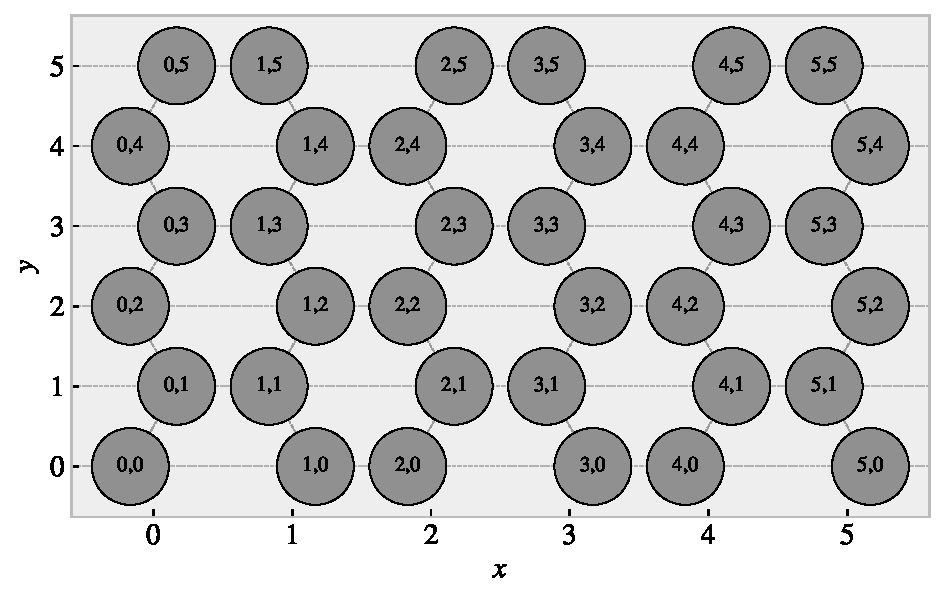
\includegraphics[width=0.7\linewidth]{figures/system/atom_indexing.pdf}
  \caption{Illustration of the graphene atom site indexing. The x-coordinate increment along the armchair direction (pointing to zigzag chains) while the y-coordinate increment along the zigzag direction.}
  \label{fig:atom_indexing}
\end{figure}


\subsection{Removing atoms}
To simplify the formulation of the cut patterns, we introduce the \textit{center element} which is placed in each gap of the hexagonal honeycomb structure. This is shown in~figure~\cref{fig:center_indexing}. These are not populated by any atoms but will serve as a reference for the algorithmic approaches of defining a cut pattern.

\begin{figure}[h]
  \centering
  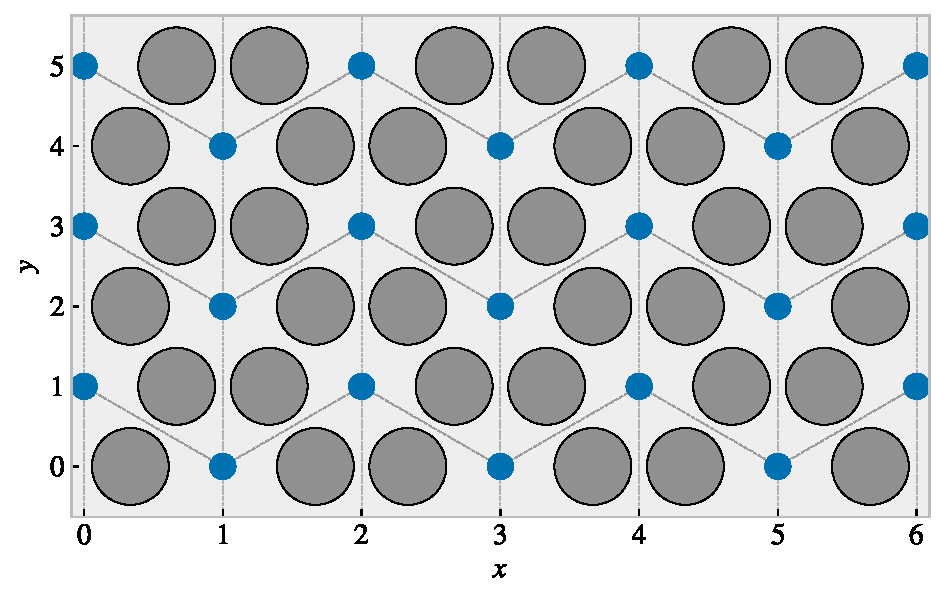
\includegraphics[width=0.7\linewidth]{figures/system/center_indexing.pdf}
  \caption{Illustration of the indexing for the introduced center element. The y-coordinate increment along the zigzag direction (pointing to armchair chains) while the x-coordinate increment along the armchair direction.}
  \label{fig:center_indexing}
\end{figure}

The nearest neighbors of the center element alternate with position, similar to the atom site indexing. However, this time it is only dependent on the x-coordinate position. Each center element has six nearest neighbors, in a clockwise
direction we can denote them: ``up'', ``upper right'', ``lower right'',
``down'', ``lower left'', ``upper left''. The ``up'' and ``down'' neighbors are always accessible as $(i,j\pm 1)$. However, for even $i$ the $(i+1,j)$ index corresponds to the
``lower right'' neighbour while for odd $i$ this corresponds to the ``upper
right'' neighbour. This shifting applies for all left- or right-oriented neighbors and the full neighbor list is illustrated in~\cref{fig:center_directions}. 

\begin{figure}[h]
  \centering
  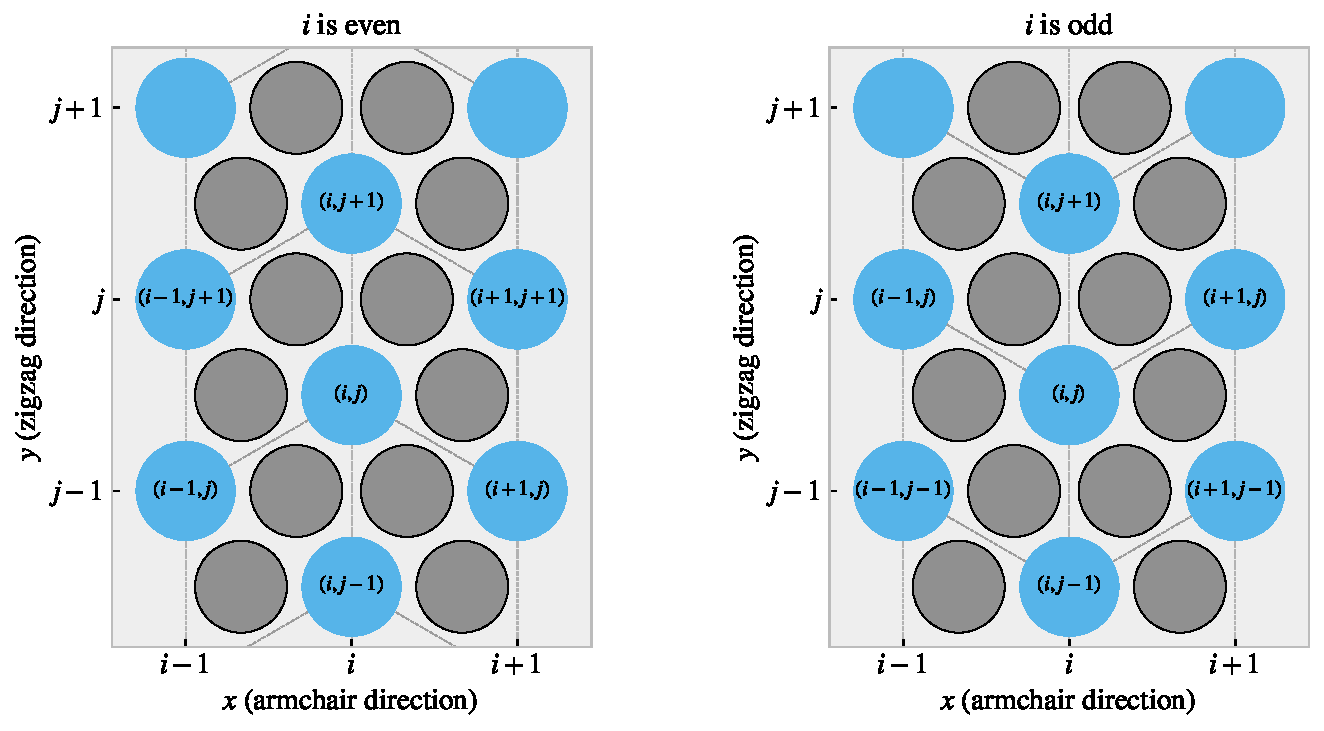
\includegraphics[width=0.7\linewidth]{figures/system/center_directions.pdf}
  \caption{Illustration of the center element neighbor indexes for the case when the x-coordinate $i$ is even (left) and $i$ is odd (right).}
  \label{fig:center_directions}
\end{figure}

We define a cut pattern by connecting center elements in connected paths. As
we walk from center element to center element we remove atoms according to one of two rules 
\begin{enumerate}
  \item Remove intersecting atoms: We remove the pair of atoms placed directly
  in the path we are walking. That is, when jumping to the ``up'' center
  element we remove the two upper atoms located in the local hexagon of atoms.
  This method is sensitive to the order of the center elements in the path. 
  \item Remove all surrounding atoms: We simply remove all atoms in the local
  hexagon surrounding each center element. This method is independent of the
  ordering of center elements in the path.
\end{enumerate}
We notice that removing atoms using either of these rules will not guarantee an injective, one-to-one, mapping. The first rule, being path dependent, will more often result in a unique result. However, for both methods, it is possible to construct two different paths leading to the same cut pattern as shown in the following example:
\begin{align*}
  \text{Path 1:} \quad (i, j) &\rightarrow \underbrace{(i+1,j+1)}_{\text{upper right}} \rightarrow \underbrace{(i, j+1)}_{\text{up}} \rightarrow \underbrace{(i+1, j+2)}_{\text{upper right + up}} \rightarrow \underbrace{(i+1, j+1)}_{\text{upper right}} \\
  \text{Path 2:} \quad (i, j) &\rightarrow \underbrace{(i+1,j+1)}_{\text{upper right}} \rightarrow \underbrace{(i+1, j+2)}_{\text{upper right + up}} \rightarrow \underbrace{(i, j+1)}_{\text{up}}
\end{align*}
\hl{Illustrate the example path, because I think it is otherwise impossible to follow.}

For the second rule, it is even more obvious that different paths can result in the same final pattern. For instance, if we incircle a center element completely there will be no surrounding atoms left to remove when jumping to that center element. This highlights the motivation for defining the atom-based indexing system which yields an injective mapping between the binary matrix and the graphene lattice. However, using the center elements as a reference makes it easier to design the cut patterns since we can always go in one of the six directions defined by the center element neighbors. In contrast, the atom indexing system has alternating directions for its neighbors, making it more complicated to define cut patterns.
 

\section{Kirigami patterns}
We propose a series of Kirigami-inspired cut patterns for the altering of the graphene sheet. We seek inspiration from macroscale patterns that showcases a considerable amount of out-of-plane buckling when stretched. We choose to imitate two different designs: 1) An alternating repeating series of perpendicular cuts as shown in~\cref{fig:kirigami_inspiration_a} popularly used in studies of morphable metematerials~\cite{new_pop_up}. This pattern produces surface buckling with a tetrahedron (three-sided pyramid) shape when stretched. 2) A more intricate pattern shown in~\cref{fig:kirigami_inspiration_b} which is used commercially by Scotch\textsuperscript{TM} Cushion Lock\textsuperscript{TM} \cite{cushion_wrap} as protective wrap for items during shipping. This pattern buckles into a hexagonal honeycomb structure when stretched. In addition to the modeling of the so-called \textit{Tetrahedron} and \textit{Honeycomb} patterns, we also create a series of random walk patterns.

\begin{figure}[h]
  \centering
  \begin{subfigure}[t]{0.48\textwidth}
      \centering
      \includegraphics[width=\textwidth]{figures/system/pop_up_inspiration.png}
      \caption{}
      \label{fig:kirigami_inspiration_a}
    \end{subfigure}
    \hfill
    \begin{subfigure}[t]{0.48\textwidth}
      \centering
      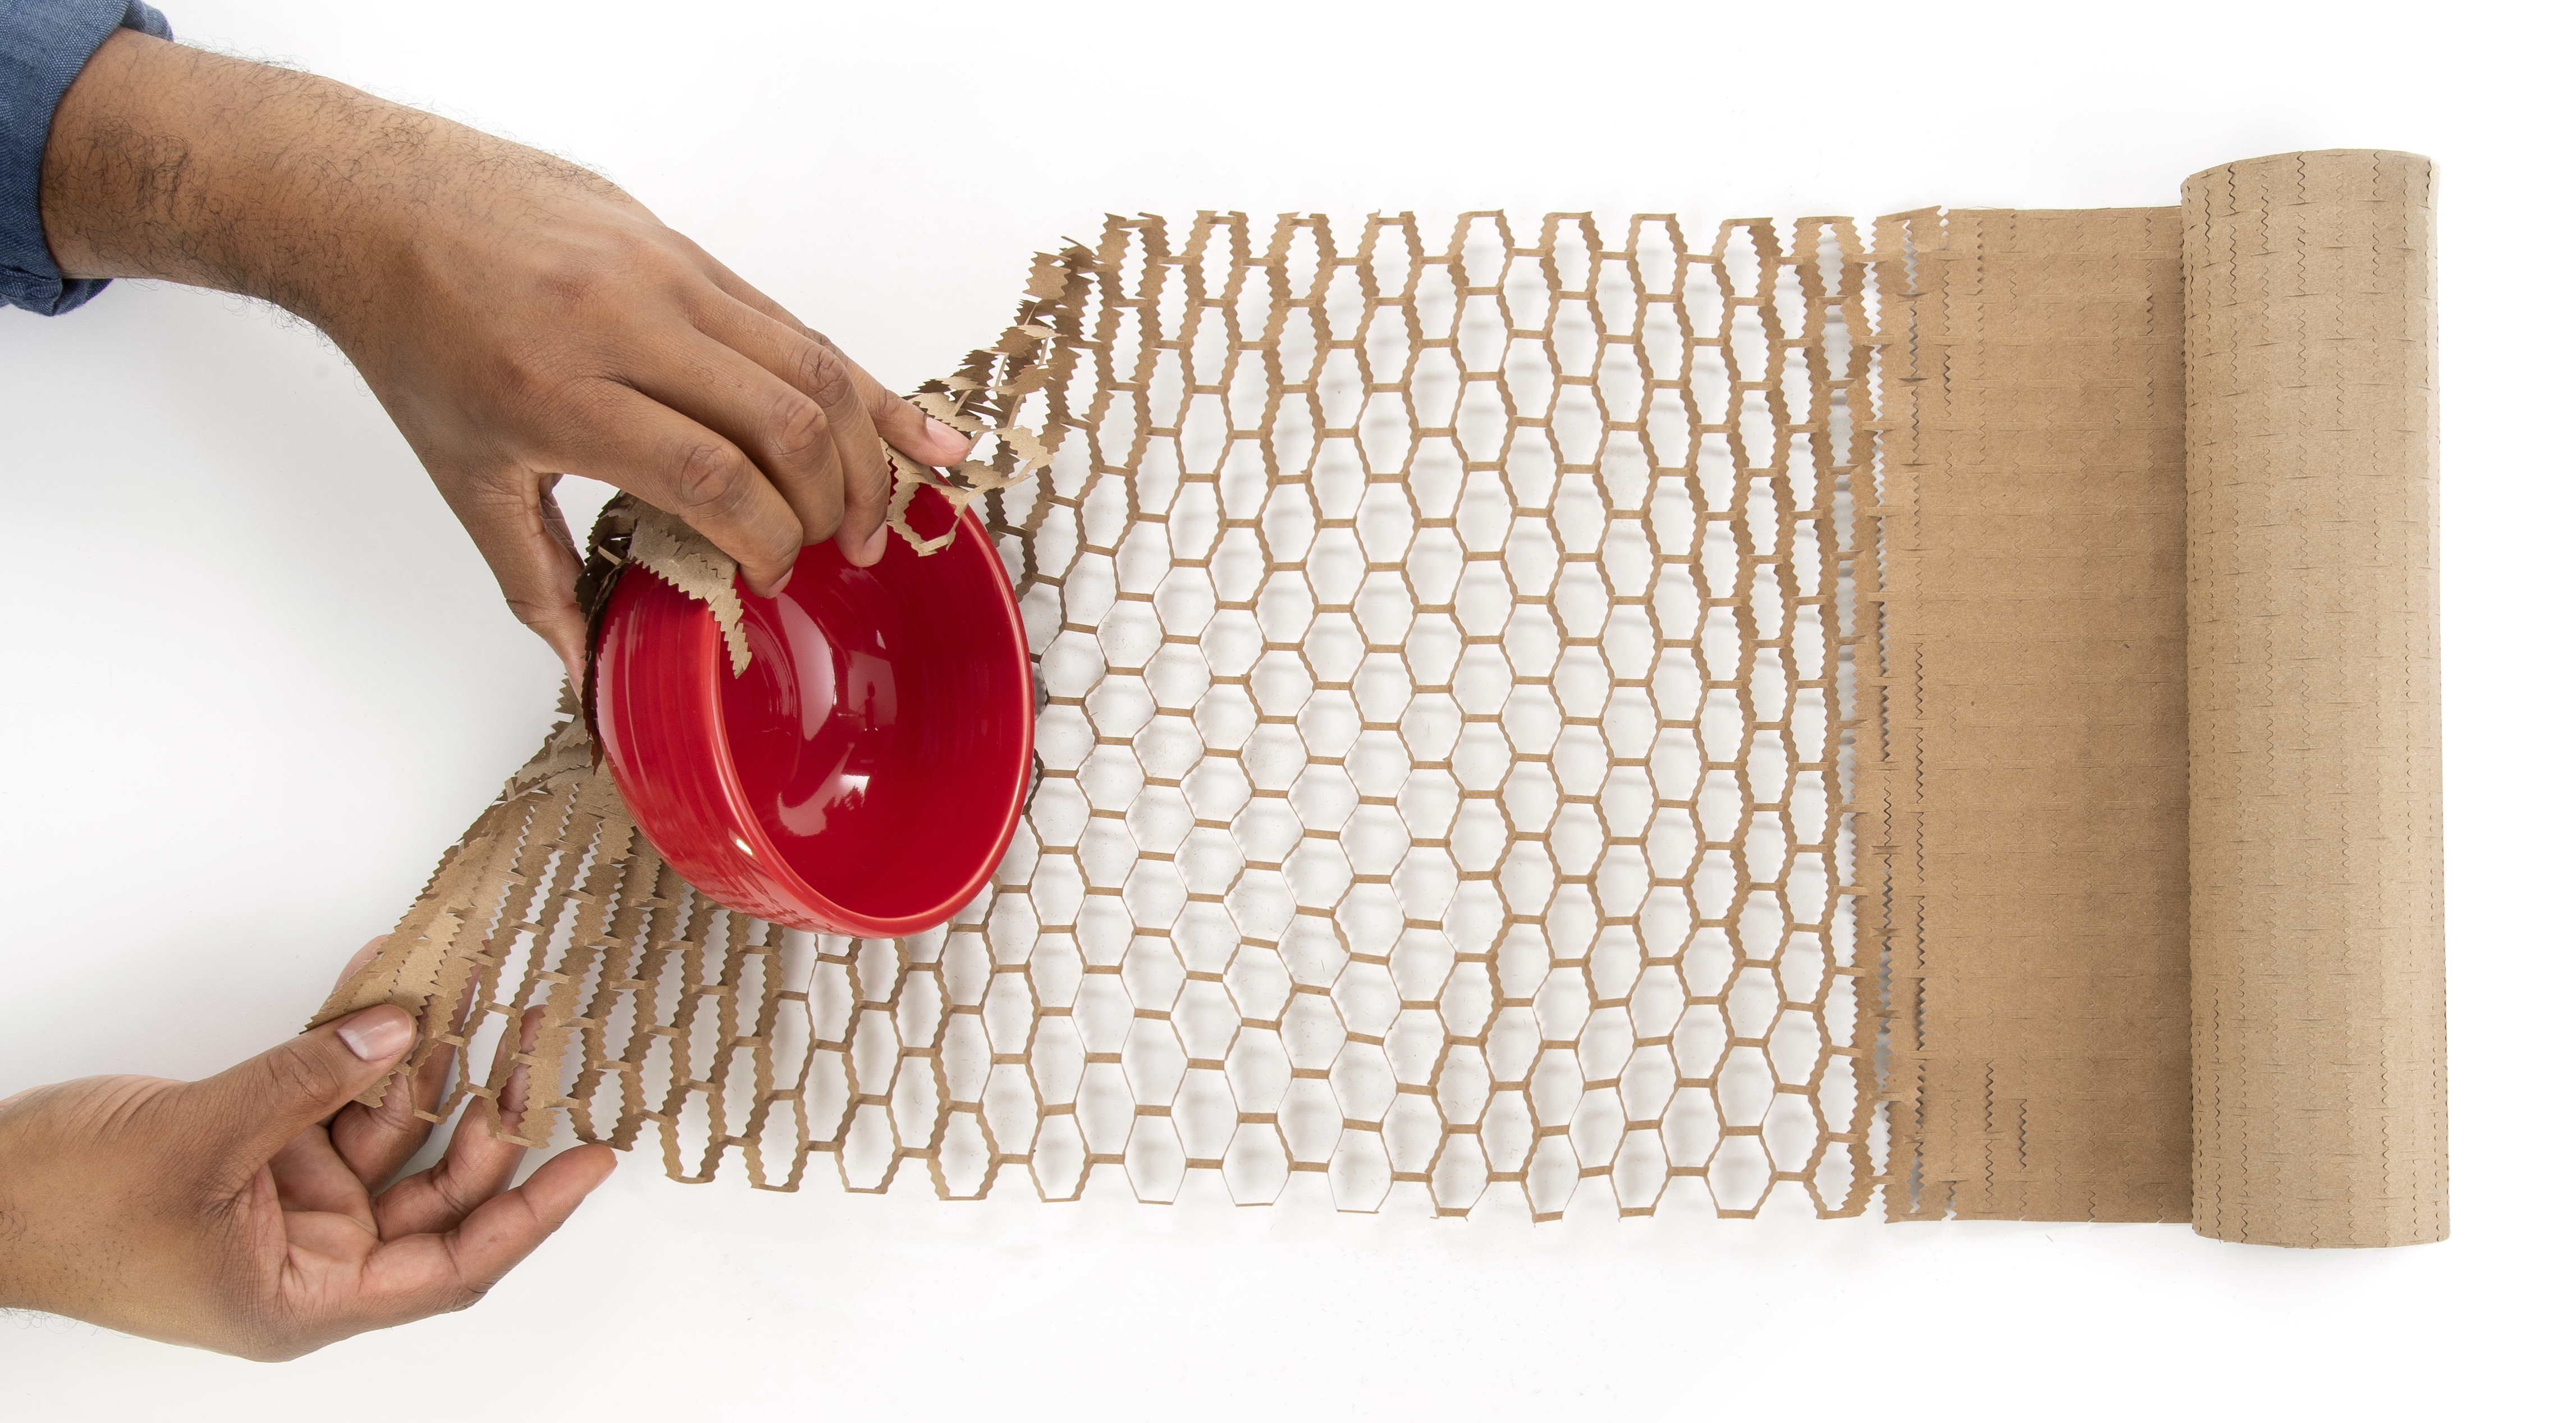
\includegraphics[width=\textwidth]{figures/system/honeycomb_inspiration.jpg}
      \caption{}
      \label{fig:kirigami_inspiration_b}
  \end{subfigure}
  \hfill
     \caption{Macroscale kirigami cut patterns used as inspiration for the nanoscale implementation. (a) Tetrahedron: Alternating perpendicular cuts producing a tetrahedron shaped surface buckling when stretched. Reprinted from~\cite{new_pop_up}. (b) Honeycomb: Scotch\textsuperscript{TM} Cushion Lock\textsuperscript{TM} \cite{cushion_wrap} producing a honeycomb-shaped surface buckling when stretched.}
     \label{fig:kirigami_inspiration}
\end{figure}

\subsection{Tetrahedron}
The \textit{Tetrahedron} pattern is defined in terms of center elements for
which all atoms surrounding a given center element are removed. The pattern
consists of two straight cuts, referred to as line 1 and line 2, that are
arranged perpendicular to each other. The lines are positioned such that the
center of one line aligns with the other line, and with a given spacing in
between. This is illustrated in~\cref{fig:pop_up}. In order to achieve
perpendicular cuts we cannot rely purely on the six center element directions
corresponding to the center element neighbors which are spaced by 60$^\circ$. We
let line 1 run along the center elements in the direction of the ``upper right''
(and ``lower left'') center elements, while line 2 goes in the direction between
the ``down'' and ``lower right'' (``up'' and ``upper left'') center elements,
corresponding to the direction $(1/\sqrt{3}, -1)$. We define variations of the
pattern by the number of center elements $L_1$ and $L_2$ in line 1 and 2
respectively, together with the spacing between the lines $d$, as the tuple
$(L_1, L_2, d)$. The pattern is constructed by translating the two lines to the
whole sheet according to the spacing. Due to the alignment criteria of having
one line point to the center of the other line, we can only allow an odd line
length. Furthermore, in order to ensure that each center element is translated
to an $i$-index of similar odd or evenness, we must in practice require that
$|L_2 - L_1| = 2, 6, 10, \ldots \ $. \cref{fig:pop_up} shows a visual
representation of the pattern components for the $(7, 5, 2)$ patteren. 


\begin{figure}[h]
  \centering
  \begin{subfigure}[t]{0.48\textwidth}
      \centering
      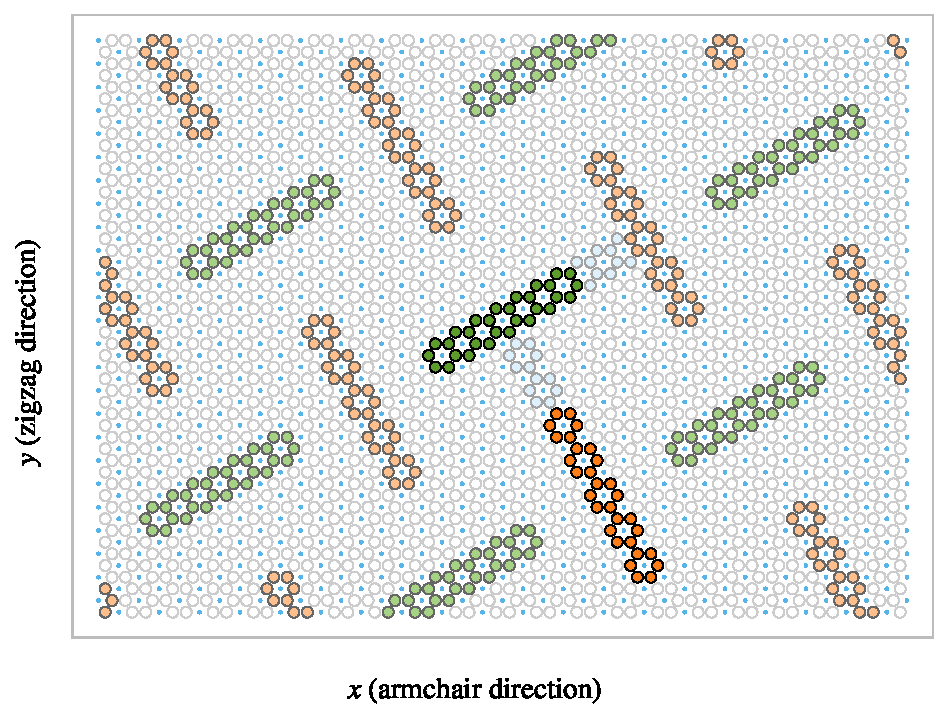
\includegraphics[width=\textwidth]{figures/system/pop_up_inverse.pdf}
      \caption{}
      \label{fig:pop_up_a}
    \end{subfigure}
    \hfill
    \begin{subfigure}[t]{0.48\textwidth}
      \centering
      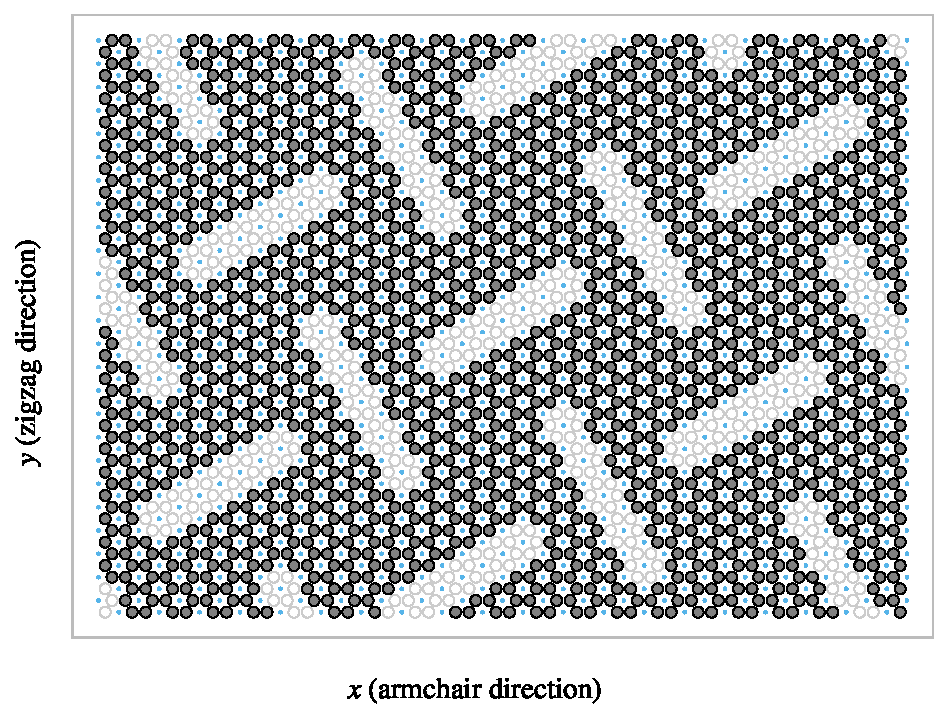
\includegraphics[width=\textwidth]{figures/system/pop_up_pattern.pdf}
      \caption{}
      \label{fig:pop_up_b}
  \end{subfigure}
  \hfill
     \caption{Visual representation of the Tetrahedron pattern consisting of two perpendicular lines, line 1 and line 2, of length $L_1$ and $L_2$ respectively, with spacing $d$. This example uses $(L_1, L_2, d) = (7, 5, 2)$ and a sheet matrix size $40 \times 50$ corresponding to 2000 atom sites and an approximate sheet size of $84 \times \SI{77}{\text{Å}}$. The non-filled circles represent the possible atom site positions and the blue dots are the center elements. (a) Highlights the removed atoms in the pattern. Line 1 is shown in green and line 2 in orange, with lighter colors for the translated variations. The spacing is indicated in light blue. (b) The sheet after applying the cut pattern with grey circles denoting present atoms.}
     \label{fig:pop_up}
\end{figure}

In addition to the three parameters $L_1, L_2, d$, the pattern is also anchored
to a reference point that describes the position of line 1 and line 2 before
being translated to span the sheet. Due to the repeating structure of the
pattern, there exist a small finite number of unique reference positions. For
the pattern $(7, 5, 2)$ used as an example in~\cref{fig:pop_up}, there are
140\footnote{The general formula for calculating this number is rather
complicated in comparison to its importance in this context. Therefore, we have
omitted the formula and only provide the numerically backed result for the
specific parameter set. The derivation of the formula was also deemed not to be
rigorous enough.} unique reference points. Some additional variation of the
pattern is showcased in~\cref{fig:pop_up_flavors} each with a reference position
at the center of the sheet. Note that a smaller sheet size is used in
both~\cref{fig:pop_up} and ~\cref{fig:pop_up_flavors} for illustrative purposes.

\begin{figure}[h]
  \centering
  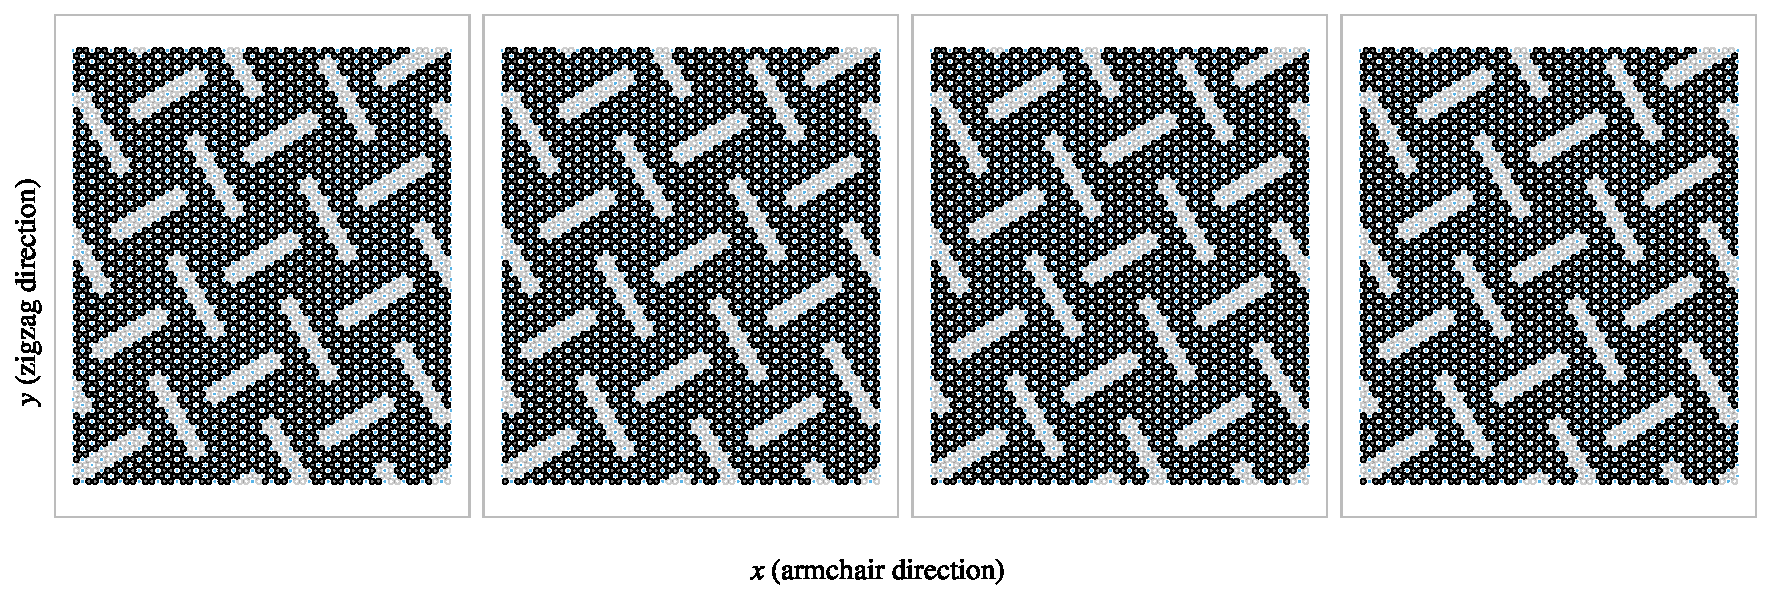
\includegraphics[width=\linewidth]{figures/system/pop_up_flavors.pdf}
  \caption{Example of different Tetrahedron cut pattern variations. The specific parameters are noted as titles and all of the patterns use the center of the sheet as a reference position. The circles in the figure represent atom sites, where grey-filled circles indicate the presence of atoms and transparent circles indicate removed atoms. The blue dots in the figure indicate the center elements The sheet matrix size is $40 \times 80$ corresponding to 3200 atom sites and an approximate sheet size of $84 \times \SI{123}{\text{Å}}$.}
  \label{fig:pop_up_flavors}
\end{figure}


\subsection{Honeycomb}
The \textit{Honeycomb} pattern is defined, similarly to the Tetrahedron pattern,
in terms of the center elements for which all surrounding atoms are removed. The
Honeycomb pattern is built from a repeating series of cuts reminiscent of the
Roman numeral one rotated by 90$^{\circ}$
(\rotatebox[origin=c]{90}{\MakeUppercase{\romannumeral 1}}). For a given spacing
these are put next to each other in the x-direction,
\rotatebox[origin=c]{90}{\MakeUppercase{\romannumeral 1}}
\rotatebox[origin=c]{90}{\MakeUppercase{\romannumeral 1}}
\rotatebox[origin=c]{90}{\MakeUppercase{\romannumeral 1}}, to achieve a row
where only a thin \textit{bridge} in between is left to connect the sheet
vertically in the y-direction. By placing multiple rows along the y-direction
with alternating x-offset we get the class of honeycomb patterns as visualized
in~\cref{fig:honeycomb}. The pattern is described in terms of the parameters:
(x-width, y-width, bridge thickness, bridge length) which is annotated
in~\cref{fig:honeycomb_a} with the parameters (2, 2, 1, 5) used as an example.
Some additional variations of the pattern class are showcased
in~\cref{fig:honeycomb_flavors}.


\begin{figure}[h]
  \centering
  \begin{subfigure}[t]{0.48\textwidth}
      \centering
      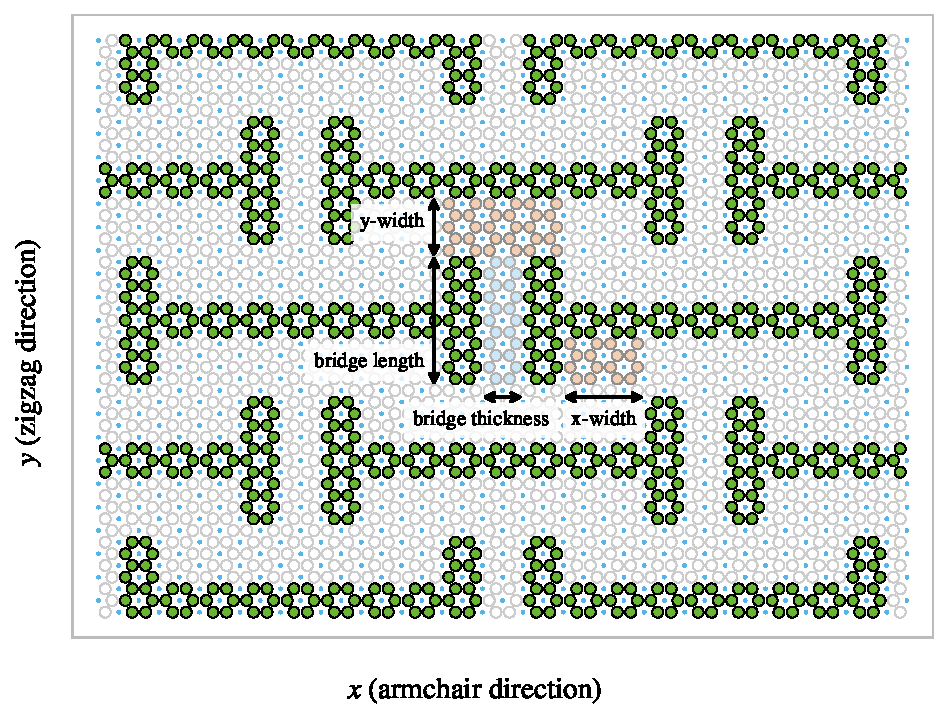
\includegraphics[width=\textwidth]{figures/system/honeycomb_inverse.pdf}
      \caption{}
      \label{fig:honeycomb_a}
    \end{subfigure}
    \hfill
    \begin{subfigure}[t]{0.48\textwidth}
      \centering
      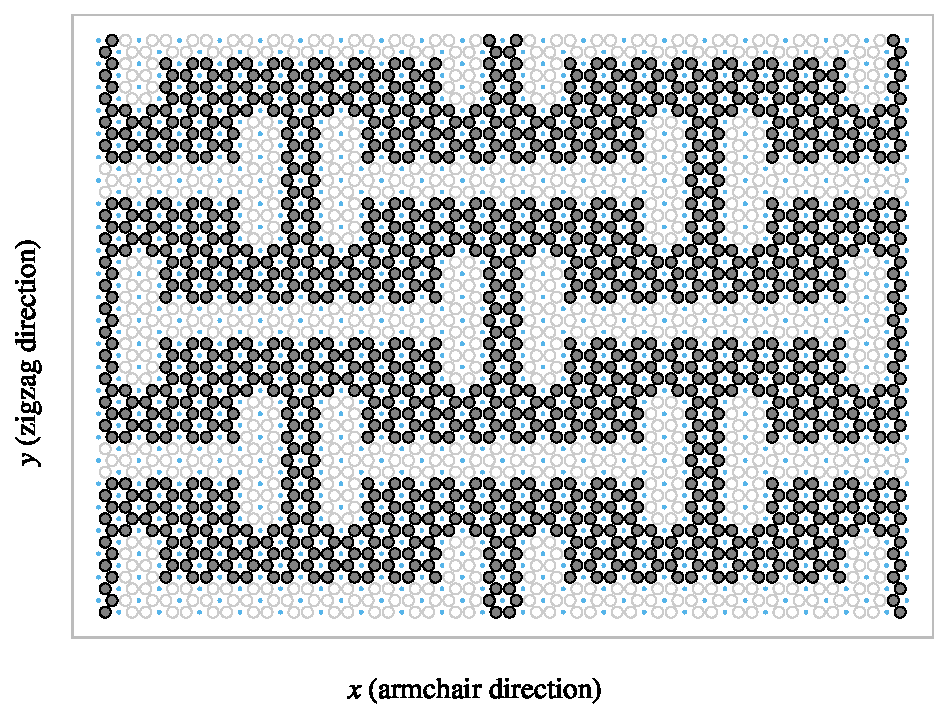
\includegraphics[width=\textwidth]{figures/system/honeycomb_pattern.pdf}
      \caption{}
      \label{fig:honeycomb_b}
  \end{subfigure}
  \hfill
     \caption{Visual representation of the Honeycomb pattern defined by the (x-width, y-width, bridge thickness, bridge length) parameters as annotated on the figure. This example uses the parameters $(2,2,1,5)$ and a sheet matrix size $40 \times 50$ corresponding to 2000 atom sites and an approximate sheet size of $84 \times \SI{77}{\text{Å}}$. The non-filled circles represent the possible atom site positions and the blue dots are the center elements. (a) Highlights the removed atoms in the pattern with annotations for the four defining parameters. (b) The sheet after applying the cut pattern with grey circles denoting present atoms. }
     \label{fig:honeycomb}
\end{figure}


\begin{figure}[h]
  \centering
  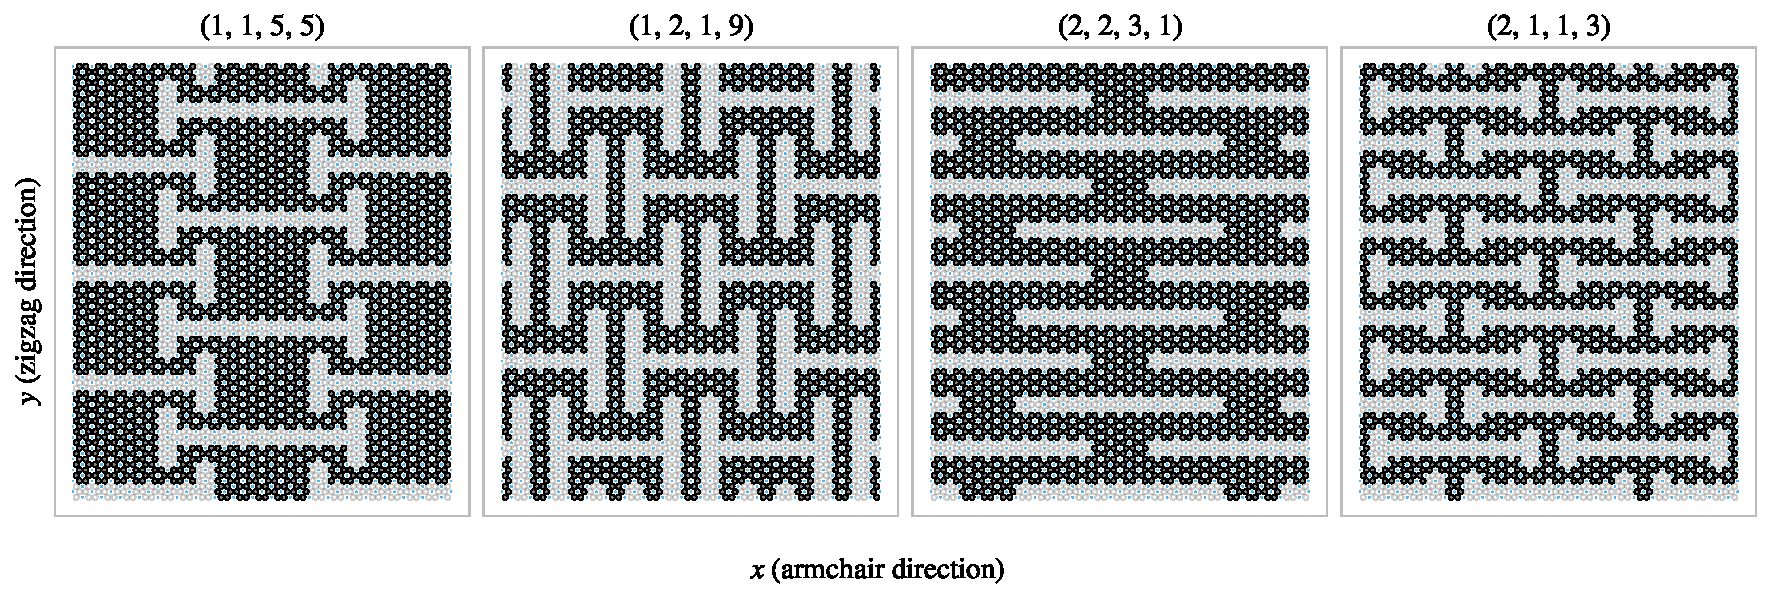
\includegraphics[width=\linewidth]{figures/system/honeycomb_flavors.pdf}
  \caption{Example of different Honeycomb cut pattern variations. The specific parameters are noted as titles and all of the patterns use the center of the sheet as a reference position. The circles in the figure represent atom sites, where grey-filled circles indicate the presence of atoms and transparent circles indicate removed atoms. The blue dots in the figure indicate the center elements. 
  The sheet matrix size is $40 \times 80$ corresponding to 3200 atom sites and an approximate sheet size of $84 \times \SI{123}{\text{Å}}$.}
  \label{fig:honeycomb_flavors}
\end{figure}



\subsection{Random walk}
The random walk serves as a method for generating Kirigami patterns with ranomized features. The motivation for doing this is to create an ensemble of patterns that populate the configuration space more broadly than the more systematic patterns described earlier. This is thought to be important for the quality of the dataset used for machine learning. By this argument, a straightforward way to create random configurations could be achieved simply by random noise, either uniform or Gaussian. However, this would often leave the sheet detached with lots of non-connected atom clusters. Intuitively, we do not find this promising for the generation of large-scale structures which we hypothesize to be of interest. The random walk pattern generation is characterized by the parameters summarized in ~\cref{tab:RW_params} which will be introduced throughout the following paragraphs. 

\begin{table}[h]
  \begin{center}
  \caption{Parameters for the random walk generator.}
  \label{tab:RW_params}
  \begin{tabular}{ | c | c | m{8cm} |} \hline
  \textbf{Parameters} & \textbf{Value} & \textbf{Description}  \\ \hline
  Num.\ walkers ($M$) & Integer $\ge$ 1 & Number of random walks to be initiated on the sheet (one at a time). \\ \hline
  Max.\ steps ($S$)  & Integer $\ge$ 1 &The maximum steps allowed for any random walker. \\ \hline
  Min.\ distance  & Integer $\ge$ 0 &The minimum distance required between any future paths and the previous paths in terms of the shortest walking distance in between. \\ \hline
  Bias  & (direction, strength $\ge0$) & Bias direction and strength defining the discrete probability for the choice of the next site. \\ \hline
  Connection  & Atoms / Center elements & Whether to walk between atom sites or center elements removing all adjacent atoms. \\ \hline
  Avoid invalid  & True/False & Whether to remove already visited sites from the neighbor list before picking the next site. This prevents jumping to already visited sites and lowers the likelihood of early termination.  \\ \hline
  Stay or break  & $p = [0,1]$ & Probability that the walker will maintain its direction for the next step. \\ \hline
  Periodic  & True/False & Whether to use periodic boundary conditions on all four sides. \\ \hline
  Avoid clustering  & Integer $\ge$ 0 & Amount of times to restart the whole random walk generation in order to arrive at a non-detached configuration. If no valid configuration is reached after this amount of tries, the non-spanning clusters are removed.\\ \hline
  RN6  & True/False & Randomly change the bias direction between the deployment of each random walker to one of the six center element directions. \\ \hline
  Grid start  & True/False & The option to have the random walkers start in an evenly spaced grid. \\ \hline
  Centering  & True/False & Relocate the path of a random walk after termination such that the path center of mass gets closer to the starting point (without violating the rules regarding already visited sites).\\ \hline
  \end{tabular}
  \end{center}
\end{table}

\subsubsection{Fundamentals} % M, S, Connection, Periodic, Avoid invalid
For an uncut sheet, we deploy $M$ random walkers, one at a time, and let them
walk for a maximum number of $S$ steps. We can either let the walker travel
between atom sites, removing the atoms in the path as it goes, or between the
center elements, removing all surrounding atoms. This is managed by setting the
\textit{connection} parameter to either \textit{atom} or \textit{center
elements}. The method of removing only the intersecting atoms between center
elements was also incorporated, but we ended up not using it due to plenty of
other interesting options. Nonetheless, we will always remove a site once
visited such that the walker itself, or any other walkers, cannot use this site
again. This leads to a self-avoiding random walk, meaning that the walker does
not cross its own path. However, it furthermore constrains the walkers to avoid
the path taken by any previous walker, and thus we might denote this property as
``other avoiding''. By default, the walker has an equal chance of choosing any
of its adjacent neighbors for the next step, i.e.\ we draw the next step from a
discrete uniform distribution. Optionally we can use periodic boundary
conditions, by setting the parameter \textit{periodic} to true or false,
allowing neighboring sites to be connected through the edge in both the x and
y-direction. When traveling on atom sites this ensures that we have three
neighbor options for the next step while traveling on the center elements this
gives six neighbor options. If the walker happens to arrive at an already
visited site the walk is terminated early. Optionally, we can choose to remove
any neighboring sites already visited from the neighbor list and choose
uniformly between the remaining options instead. This is done by setting the
parameter \textit{avoid invalid} to true. This prolongs the walking distance,
but the walker is still able to find itself in a situation where no neighboring
sites are available. Note that the walker is not allowed to backtrack its own
path either, and thus in such a case the walk will be terminated despite the
setting of \textit{avoid invalid}.


\subsubsection{Spacing of walking paths} % minimum distance
To control the spacing between the paths of the various walkers, we implement a so-called \textit{minimum distance} parameter, taking integer values $\ge 0$. This parameter describes the minimum spacing required between paths in terms of the least amount of walking steps. When a walker has ended its walk, either by early termination or hitting
the maximum limits of steps, all sites within walking distance of the minimum
distance are marked as visited, although they are not removed from the sheet.
This prevents any subsequent walkers to visit those sites in their walk
according to the general behavior introduced in the previous paragraph. In
practice, this is done through a recursive algorithm as described in ~\cref{algo:walk_dis}. For a given path the function \textit{walk\_distance()} is called with the input being a list of all sites in the given paths. The function gathers all the neighbors of each site, regardless of their state on the sheet. It then calls itself recursively using this neighbor list as input, while incrementing a distance counter that is also passed along as an argument. This results in an expansion along all possible outgoing paths from the initial path of interest. Once the distance limit is reached, the function returns the final neighbor lists, which are then accumulated into a final output. This output corresponds to a list of all sites within the minimum distance to the path.


\begin{algorithm}[h]
  \caption{Recursive algorithm implemented as a class method of the random walk generator. For a given path input it flags all sites within a distance given by the class attribute \textit{self.min\_dis}.}
  \label{algo:walk_dis}
  \begin{algorithmic}[1]
    \Require self.min\_dis $>$ 0 
    \Function{walk\_distance}{self, input, dis = 0, pre = [ ]}
      % \State neigh $\gets$ NewList() 
      \State new\_neigh $\gets$ [ ] \Comment{Initialize list for new neighbors}
      \For{site in input}
        \State neigh $\gets$ get\_neighboring\_sites(site) \Comment{Get surrounding neighbors}
        \For{n in neigh}
          \If {(n not in pre) and (n not in new\_neigh)} \Comment{If not already added}
            \State AddItem(new\_neigh, n) \Comment{then add the site}
          \EndIf
        \EndFor
      \EndFor
      \State dis += 1 \Comment{Increment distance counter}
      \If{dis $\ge$ self.min\_dis} \Comment{Max limit hit}
        \State \Return input + new\_neigh 
      \Else \Comment{Start a new walk from each of the neighboring sites}
        \State pre $\gets$ input
        \State \Return pre +  self.walk\_distance(new\_neigh, dis, pre)
      \EndIf
    \EndFunction
  \end{algorithmic}
\end{algorithm}


\subsubsection{Bias} % Bias
We provide the option to perform a biased random walk by specifying the
\text{bias} parameter, which consists of a direction and a strength. To achieve
this, we model each step of the walk analog to a system in the canonical
ensemble under the influence of an external force $\vec{F}$ representing the
bias. For such a system each microstate $i$, corresponding to the sites in the
neighbor list, has the associated probability $p_i$ given by the Gibbs–Boltzmann
distribution
\begin{align*}
  p_{i} = \frac{1}{Z}e^{-\beta E_i}, \qquad Z = \sum_i e^{-\beta E_i},
\end{align*}
where $Z$ is the canonical partition function, $\beta = 1/k_B T$ for the
boltzmann constant $k_B$ and temperature $T$, and $E_i$ the energy of site $i$.
We model the energy of each site as the work required to move there. For a step
$\vec{s}$ the energy becomes $E_i = -\vec{s}\cdot\vec{F}$, where the sign is chosen such that the energy (difference) is negative when moving along the bias, analogous to an energy gain by
moving there. Due to the symmetry of the random walk sites, both the atom sites and the center elements, the step length to neighboring sites will always be equal. By defining
the bias strength $B = \beta|\vec{F}||\vec{s}|$ we get that the probability for
jumping to site $i$ is
\begin{align*}
  p_i = \frac{1}{Z}e^{B\hat{\vec{s}}\cdot\hat{\vec{F}}} \propto e^{B\hat{\vec{s}}\cdot\hat{\vec{F}}},
\end{align*}
 where the hat denotes the unit vector. The bias strength $B$ then captures the opposing effects of the magnitude of the external force and the
 temperature of the system since $B\propto |\vec{F}|/T$. We notice that
 $\hat{\vec{s}}\cdot\hat{\vec{F}} = \cos{(\theta)}$ for the angle
 between the step and bias direction $\theta$. This shows that the bias will have the
 biggest positive contribution to the probability when the step direction is fully aligned with the bias
 direction ($\theta = 0$), have no contribution for orthogonal directions
 ($\theta = \pm \pi/2$) and the biggest negative contribution when the directions
 are antiparallel ($\theta = \pi$). The partition function serves simply as a
 normalization constant. Thus, numerically we can enforce this simply by setting $Z = 1$ at first, calculating $p_i$, and then normalizing the result at the final stage as a
 division by the sum of all $p_i$. In the numerical implementation, we then pick
 the next step by the weighted discrete probability distribution $p_i$. In~\cref{fig:bias_prob} we have illustrated how a bias of different strengths impacts the probability distribution for a random walk between center elements. We can visually confirm that the bias will favor the directions that lie close to the bias direction. This preference is more distinct at high bias strengths while at low strength $B\to0$ we get a uniform distribution that aligns with the default unbiased random walk. 

\begin{figure}[h]
  \centering
  \begin{subfigure}[t]{0.48\textwidth}
      \centering
      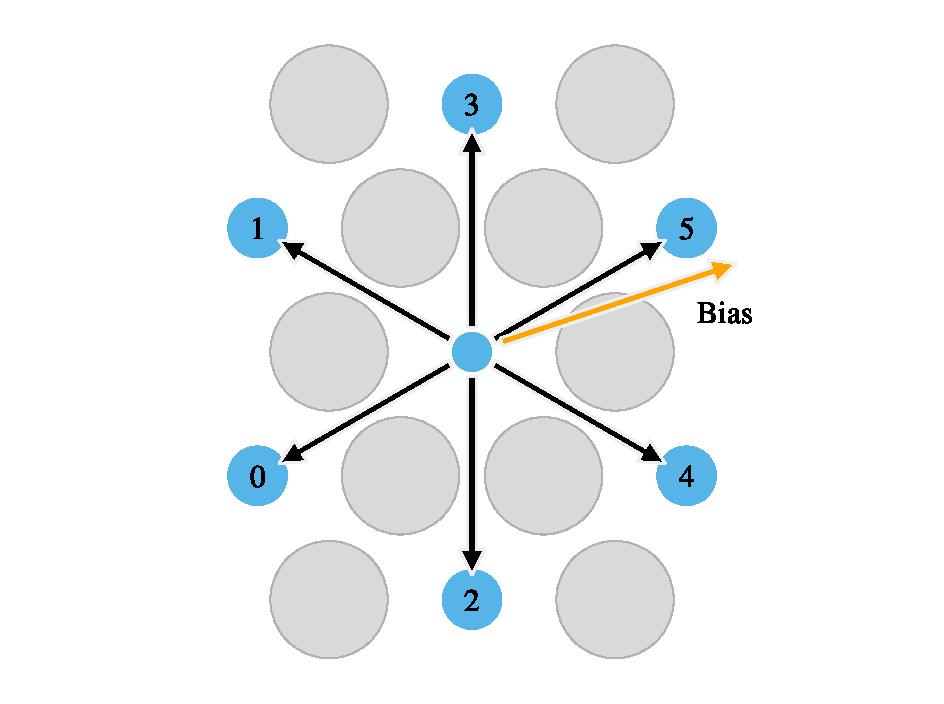
\includegraphics[width=\textwidth]{figures/system/bias_prob_a.pdf}
      \caption{}
      \label{fig:bias_prob_a}
    \end{subfigure}
    \hfill
    \begin{subfigure}[t]{0.48\textwidth}
      \centering
      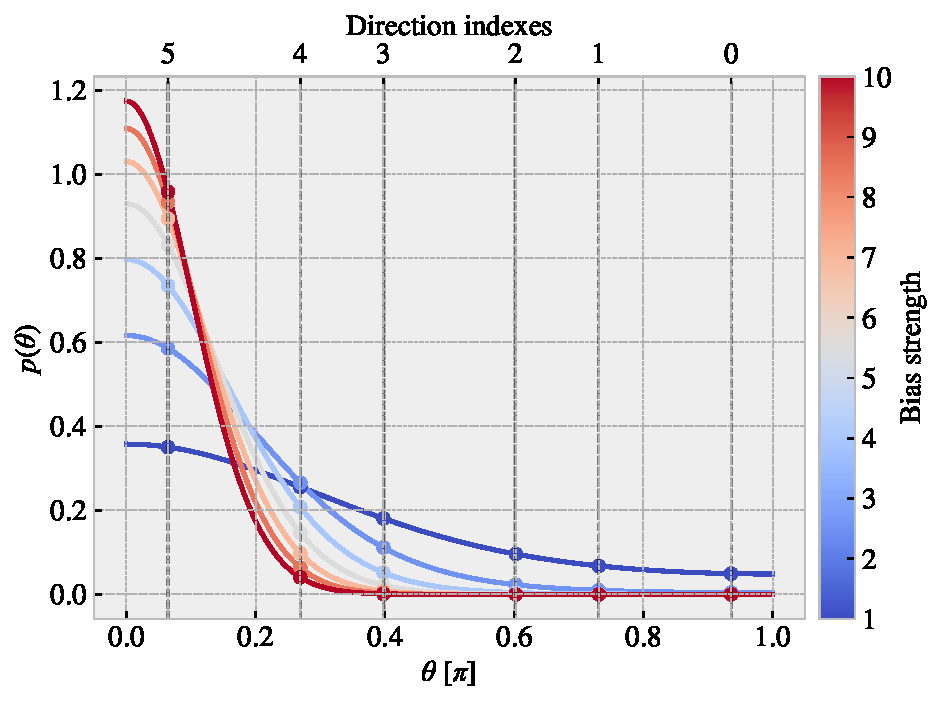
\includegraphics[width=\textwidth]{figures/system/bias_prob_b.pdf}
      \caption{}
      \label{fig:bias_prob_b}
  \end{subfigure}
  \hfill
     \caption{Illustration of the probability distribution for the various step directions during a biased random walk between center elements. (a) The possible step directions are represented by black arrows that point towards the neighboring center elements depicted as blue circles. The bias direction is denoted by an orange arrow, and the numbering indicates the most probable direction (1) towards the least probable direction (6). The atom sites are marked as grey circles for reference. (b) The probability distribution as a function of the angle $\theta$ between the step direction and the bias direction. The distribution is normalized according to the discrete probabilities marked with dots for which the continuous line simply highlights the shape of the distribution. The direction indexes correspond to the numbering on panel (a). The color map indicates different strengths of the bias. }
     \label{fig:bias_prob}
\end{figure}


\subsubsection{Stay or break}
The \textit{stay or break} parameter defines the probability
$p_{\text{stay}}$ that the walker will keep its direction or otherwise break
into a different direction by probability $1-p_{\text{stay}}$. We implement this by altering the discrete probability used for the choice of the next step. We manually set the probability to $p_{\text{stay}}$ for the site corresponding to a continuation in the same direction. We then normalize the distribution again. This allows us to perform a biased random walk in combination with a preference for keeping direction. For the center element
walk it is trivial to determine which of the neighbor directions correspond to
a continuation of direction based on the last visited site. However, for an atom site walk, it is not possible to follow the same direction in a straight line due to the hexagonal layout of the lattice. We recall that the
nearest atom neighbor indexes alternate for each increment in the x or y index (see~\cref{eq:atom_neigh_idx}) which corresponds to the alternating neighbor directions $D$ as
\begin{align*}
  (i + j) \ \text{is even} &\rightarrow D = \left\{ \frac{a}{2}\left(\frac{-2}{\sqrt{3}}, 0\right), \frac{a}{2}\left(\frac{1}{\sqrt{3}}, 1\right), \frac{a}{2}\left(\frac{1}{\sqrt{3}}, -1\right)\right\}, \\
  (i + j) \ \text{is odd} &\rightarrow D = \left\{ \frac{a}{2}\left(\frac{2}{\sqrt{3}}, 0\right), \frac{a}{2}\left(\frac{-1}{\sqrt{3}}, 1\right), \frac{a}{2}\left(\frac{-1}{\sqrt{3}}, -1\right)\right\}.
\end{align*}
One way to mitigate this issue is to use the six directions from the center element walk as the common direction to ``stay or break'' from. As showcased in~\cref{fig:stay_or_break}, in each center element direction (black arrows) there are two possible atom site directions (red and orange arrows) that are equally close to the center element direction. The red and orange arrows represent $(i+j)$ being even or odd respectively, and we notice that these appear in pairs such that we can always determine which of the atom directions is closest to the center element direction. Following this idea we can map each center direction to an atom direction depending on the even or oddness of the position. For $p_{\text{stay}} = 1$ this results in a guaranteed zigzag motion along the center element direction that it happens to start on. 

\begin{figure}[h]
  \centering
  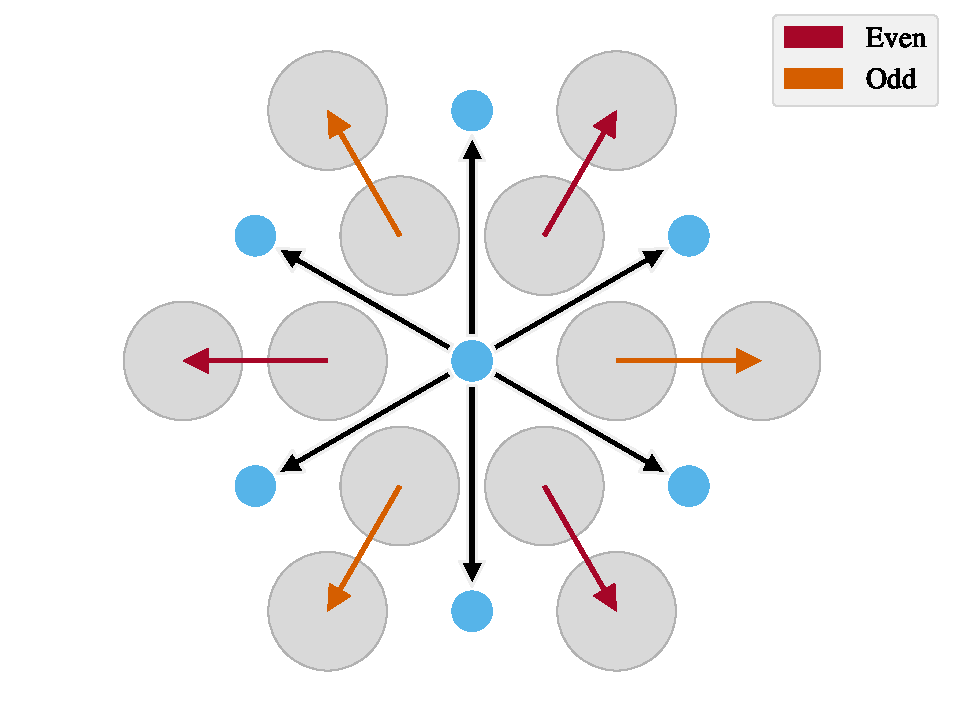
\includegraphics[width=0.5\linewidth]{figures/system/stay_or_break.pdf}
  \caption{Visualization of the center element directions (black arrows) connecting the center elements depicted as blue dots, and the atom site directions (red and orange arrows) connection the atom sites depicted as grey circles. The red arrows correspond to the case where the sum of the atom site indexes $(i,j)$ is even, while the orange arrows correspond to the case where the sum is odd. Notably, for each case, there is always one atom site direction that is uniquely closest to a given center element direction.}
  \label{fig:stay_or_break}
\end{figure}

The \textit{stay or break} feature is still subject to previously defined rules.
For instance, in the case where the preferred site is not available, the walker
will either terminate when going there, or the preferred site is removed from
the neighbor list when \textit{avoid invalid} is set to true. In the latter
case, the walker will be forced to break out of its direction and follow the new
direction that it happens to choose.


\subsubsection{Deployment schemes} % Grid start, Centering, RN6
By default, each random walker is given a uniform random starting point among
the non-visited available sites left on the sheet. This includes any
modifications in relation to the minimum distance parameter. By setting the
\textit{grid start} parameter to true, the starting points are instead
predefined on an evenly spaced grid. That is, the sheet is subdivided into the
least amount of squares that will accommodate space for each starting point. 1
walker leads to a $1\times 1$ partition, $\{2,3,4\}$ walkers lead to a $2\times
2$ partition, $\{5,6,7,8,9\}$ walker lead to a $3\times 3$ partition and so on.
For each partition square, the starting point is placed as centrally as
possible. The lower left partition square is then chosen as a default starting
place for the first walker and the remaining sites are filled according to the
order that maximizes the minimum distance between a new starting point and the
ones already used\footnote{In hindsight, it would have been less biased to
choose a random partition square as the starting one, but we do not consider
this to be of great importance for the usage of this feature in final dataset}.
An example of the deployment is shown in~\cref{fig:grid_start}.


\begin{figure}[h]
  \centering
  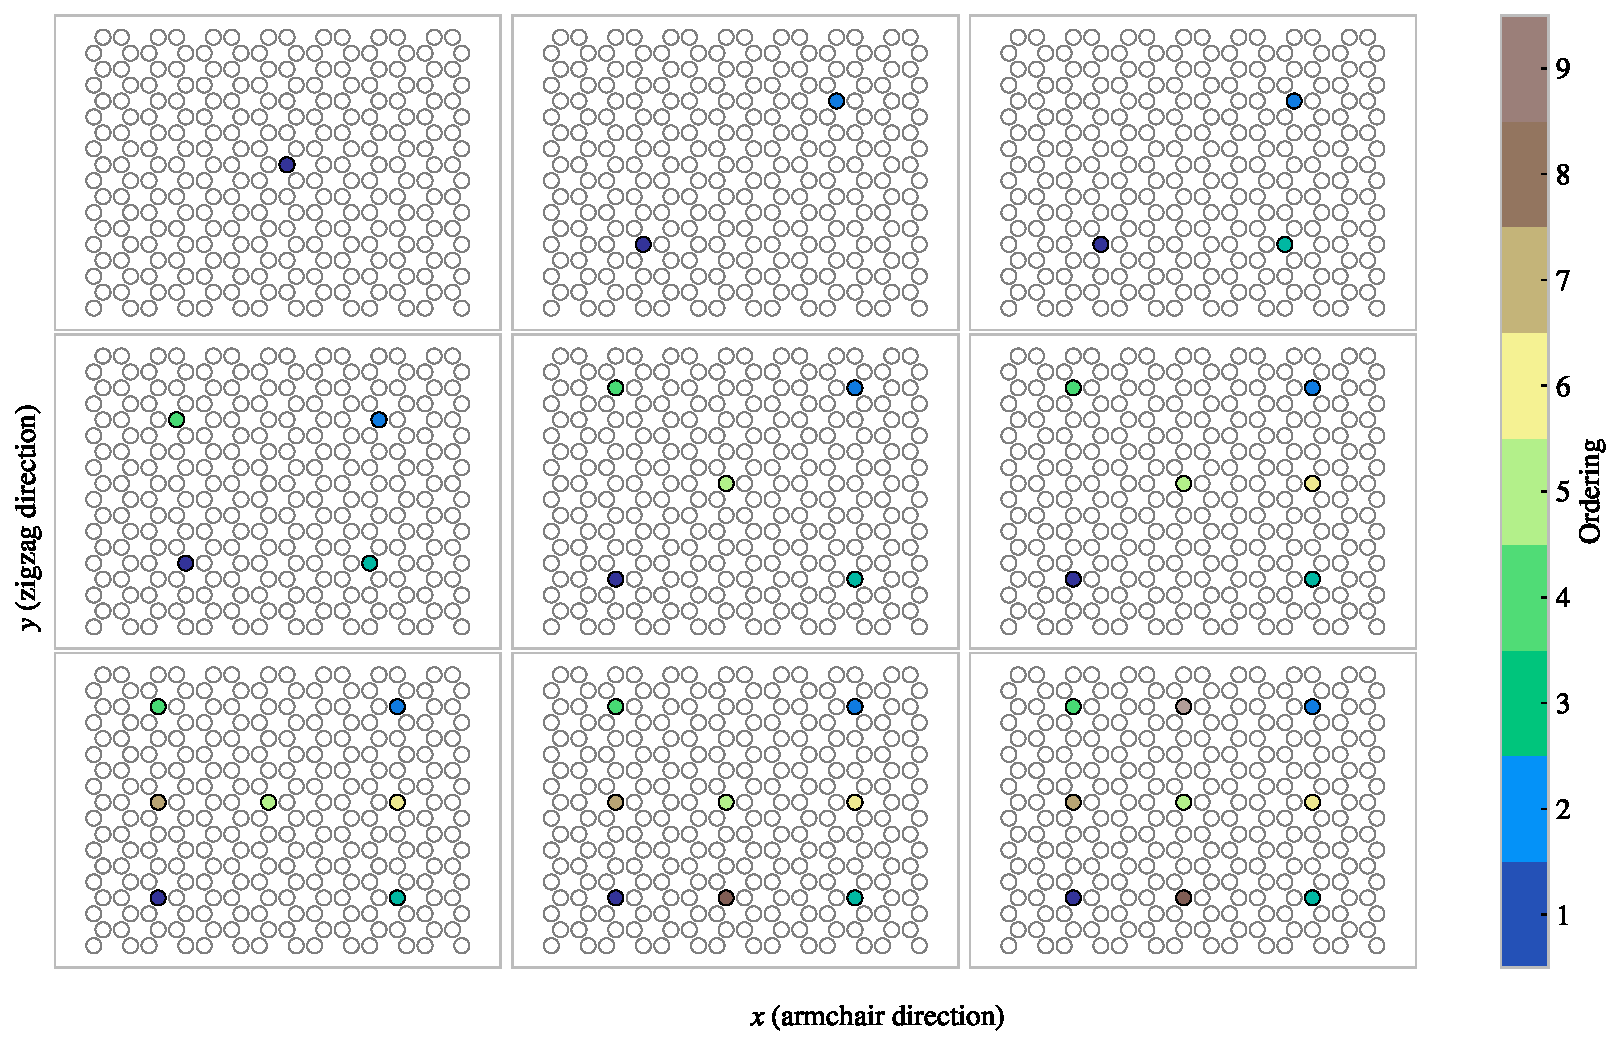
\includegraphics[width=\linewidth]{figures/system/grid_start.pdf}
  \caption{The figure illustrates the distribution of starting points when the \textit{grid start} parameter is turned on for a $14\times 18$ sheet, for varying numbers of deployed random walkers ranging from 1 to 9. The color map is used to indicate the order in which the walkers were deployed.}
  \label{fig:grid_start}
\end{figure}


The \textit{centering} parameter lets us relocate the path of the random walker
such that the path center of mass gets closer to the starting point. When
toggled on, the path is moved in the direction defined by the center of mass and
the starting point for which the closest valid relocation on the direct
translation line is chosen. This can be used in combination with the
\textit{grid start} and the \textit{bias parameter} to make rather ordered
configurations. In addition, the \textit{RN6} parameter can be used to update
the bias direction to one of the six center element directions for each new
walker deployed. This lets us create configurations like the one shown
in~\cref{fig:RW_flavors}\textcolor{red!50!black}{b}. 


\subsubsection{Validity}

The simulation procedure requires the sheet to be fully attatched, non ruptured, which can be summarized as the following requirements. 
\begin{enumerate}
  \item There exist only a single cluster on the sheet. We define a cluster as the set of atoms which can all be reached through nearest neighbour walking on the cluster.
  \item The cluster of atoms is spanning the sheet in the y-direction. This means that there exist at least one path through nearest neighbour walks that connect the bottom and the top of the sheet. This is due to the reason that the sheet must be attatched to the pull blocks.
\end{enumerate}
In order to accommodate these requirements we count the number of clusters and search for a spanning cluster after all walkers have terminated. If the requirements are not met we simply rerun the random walk from scratch. This is done according to \textit{avoid clustering} parameter which takes integer values corresponding to the number of times to repeat this process. If the requirements are not met during any of those reruns the non-spanning clusters are simply removed. In the case of no spanning cluster the configuration is skipped. This crude scheme was later reinvented as a more refined repair scheme which alters the sheet by the intention of performing the least amount of changes (addition or subtraction of atoms) in order to meet the attatchment requirements. This was done as a part of the accelerated search procedure and hence it was not utilized in the creation of the random walk dataset. 

\hl{Talk about the new repair algorithm}
\subsubsection{Random walk examples}

Some examples of the random walk patterns are illustrated in \cref{fig:RW_flavors}.

\begin{figure}[h]
  \centering
  \includegraphics[width=\linewidth]{figures/system/RW_flavors.pdf}
  \caption{Some example uses of the random walking class. \hl{Give information of parameters? Henrik says Yes :D}}
  \label{fig:RW_flavors}
\end{figure}

%
%
% Working here
%
%


% \begin{table}[H]
%   \begin{center}
%   \caption{RW flavors}
%   \label{tab:RW_flavors}
%   \begin{tabular}{ |c|c|c|c|c|c|c|} \hline
%   Fig. num. 
%   Num. walks 
%   Max Steps 
%   Min dis 
%   Bias 
%   center elem 
%   avoid invalid 
%   RN6 
%   grid start 
%   centering 
%   stay or break 
%    avoid clustering 
%    periodic \\ \hline
%   % a  num_walks = 25, max_steps = 15, min_dis = 0, bias = [direc['up_right'], 100], center_elem = False,  avoid_unvalid = False,  RN6 = False,  grid_start = True,  centering = True,  stay_or_break = 0,  avoid_clustering = 10,  periodic = True)]
%   % b  num_walks = 25, max_steps = 15, min_dis = 0, bias = [direc['up_right'], 100], center_elem = False,  avoid_unvalid = False,  RN6 = True,  grid_start = True,  centering = True,  stay_or_break = 0,  avoid_clustering = 10,  periodic = True)]
%   % c  num_walks = 20, max_steps = 30, min_dis = 4, bias = [(0,0), 0], center_elem = False,  avoid_unvalid = True,  RN6 = True,  grid_start = False,  centering = False,  stay_or_break = 0.9,  avoid_clustering = 10,  periodic = True)]
%   % d  num_walks = 30, max_steps = 40, min_dis = 4, bias = [(0,0), 0], center_elem = False,  avoid_unvalid = True,  RN6 = False,  grid_start = False,  centering = False,  stay_or_break = 0,  avoid_clustering = 10,  periodic = True)]
%   % e  num_walks = 20, max_steps = 30, min_dis = 4, bias = [direc['down_right'], 1.2], center_elem = False,  avoid_unvalid = True,  RN6 = False,  grid_start = False,  centering = False,  stay_or_break = 0,  avoid_clustering = 10,  periodic = True)]
%   % f  num_walks = 32, max_steps = 30, min_dis = 4, bias = [direc['down_left'], 1.2], center_elem = 'full', avoid_unvalid = True,  RN6 = False,  grid_start = False,  centering = False,  stay_or_break = 0,  avoid_clustering = 10,  periodic = True)]
% \end{tabular}
% \end{center}
% \end{table}
